
%\setcounter{chapter}{12}
\chapter{Neural Networks as Distribution Transformers}\label{chapter:neural_nets_as_distribution_transformers}

\pgfplotsset{
    compat=1.3,
    rep2rep axis style/.style={
            width=1.0\textwidth,
            height=1.0\textwidth,
            axis lines=bottom,
            axis line style={stealth-stealth},
            y axis line style={draw=none},
            ymajorticks=false,
            xtick distance=0.5,
            tick style={draw=none},
            xmin=0,xmax=1,
            ymin=0,ymax=1,
        },
}

\section{Introduction}
So far we have seen that deep nets are stacks of simple functions, which compose to achieve interesting mappings from inputs to outputs. This section will introduce a slightly different way of thinking about deep nets. The idea is think of each layer as a \emph{geometric transformation of a data distribution}.

\section{A Different Way of Plotting Functions}
Each layer in a deep net is a mapping from one representation of the data to another: $f: \xin \rightarrow \xout$. If $\xin$ and $\xout$ are both one-dimensional (1D), then we can plot the mapping as a function with $\xin$ on the $x$-axis and $\xout$ on the $y$-axis (\fig{\ref{fig:neural_nets_as_distribution_transformers:trad_plot}}):

%\vspace{-0.5cm}
\begin{figure}[h]
\centerline{
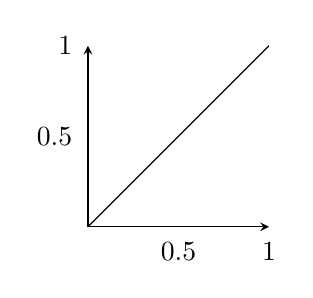
\begin{tikzpicture}
    \begin{axis}[
            width=0.32\textwidth,
            height=0.32\textwidth,
            xlabel={$\xin$},
            ylabel={$\xout$},
            axis lines=center,
            xtick distance=0.5,
            ytick distance=0.5,
            tick style={draw=none},
            xmin=0,xmax=1,
            ymin=0,ymax=1
    ]
    
    \addplot +[mark=none,smooth,black] {x};
    
    \end{axis}
\end{tikzpicture}
}
\caption{The traditional way of plotting the function $\xout = \xin$.}
\label{fig:neural_nets_as_distribution_transformers:trad_plot}
%\vspace{-0.5cm}
\end{figure}

Now, we will instead consider a different way of plotting the mapping, where we simply rotate the $y$-axis to be horizontal rather than vertical (\fig{\ref{fig:neural_nets_as_distribution_transformers:new_way_plot}}):

%\vspace{-0.5cm}
\begin{figure}[h]
\centering
\begin{minipage}[t][4.5cm][c]{0.32\textwidth}
\begin{tikzpicture}
    \begin{axis}[
            width=1.0\textwidth,
            height=1.0\textwidth,
            xlabel={$\xin$},
            ylabel={$\xout$},
            axis lines=center,
            tick style={draw=none},
            xtick distance=0.5,
            ytick distance=0.5,
            xmin=0,xmax=1,
            ymin=0,ymax=1,
    ]
    
    \addplot +[mark=none,smooth,black] {x};
    
    \addplot[scatter src=explicit symbolic, only marks, mark=triangle*, mark options={rotate=90}] coordinates {
        (0.03,0.1)
        (0.03,0.2)
        (0.03,0.3)
        (0.03,0.4)
        (0.03,0.5)
        (0.03,0.6)
        (0.03,0.7)
        (0.03,0.8)
    };
    
    \addplot[scatter src=explicit symbolic, only marks, mark=*] coordinates {
        (0.1,0)
        (0.2,0)
        (0.3,0)
        (0.4,0)
        (0.5,0)
        (0.6,0)
        (0.7,0)
        (0.8,0)
    };
    
    \addplot[mark=none,dashed] coordinates {
    	(0.1,0)
    	(0.1,0.1)
    };
    \addplot[mark=none,dashed] coordinates {
    	(0.2,0)
    	(0.2,0.2)
    };
    \addplot[mark=none,dashed] coordinates {
    	(0.3,0)
    	(0.3,0.3)
    };
    \addplot[mark=none,dashed] coordinates {
    	(0.4,0)
    	(0.4,0.4)
    };
    \addplot[mark=none,dashed] coordinates {
    	(0.5,0)
    	(0.5,0.5)
    };
    \addplot[mark=none,dashed] coordinates {
    	(0.6,0)
    	(0.6,0.6)
    };
    \addplot[mark=none,dashed] coordinates {
    	(0.7,0)
    	(0.7,0.7)
    };
    \addplot[mark=none,dashed] coordinates {
    	(0.8,0)
    	(0.8,0.8)
    };
    
    \addplot[mark=none,dashed] coordinates {
    	(0,0.1)
    	(0.1,0.1)
    };
    \addplot[mark=none,dashed] coordinates {
    	(0,0.2)
    	(0.2,0.2)
    };
    \addplot[mark=none,dashed] coordinates {
    	(0,0.3)
    	(0.3,0.3)
    };
    \addplot[mark=none,dashed] coordinates {
    	(0,0.4)
    	(0.4,0.4)
    };
    \addplot[mark=none,dashed] coordinates {
    	(0,0.5)
    	(0.5,0.5)
    };
    \addplot[mark=none,dashed] coordinates {
    	(0,0.6)
    	(0.6,0.6)
    };
    \addplot[mark=none,dashed] coordinates {
    	(0,0.7)
    	(0.7,0.7)
    };
    \addplot[mark=none,dashed] coordinates {
    	(0,0.8)
    	(0.8,0.8)
    };
    
\end{axis}
\end{tikzpicture}
\end{minipage}
\begin{minipage}[t][4.5cm][c]{0.1\textwidth}
\begin{tikzpicture}
    \draw [line width=1pt, double distance=2pt, -{Classical TikZ Rightarrow[length=2mm]}] (0,0) -- (0.5,0);
\end{tikzpicture}
\end{minipage}
\begin{minipage}[t][4.5cm][c]{0.32\textwidth}
\begin{tikzpicture}
    
    % \begin{axis}[
    %         rep2rep axis style,
    %         xlabel={$\xin$},
    %         ylabel={$\xout$},
    %         axis x line=bottom, % Place the x-axis on the bottom
    %         axis y line=top,    % Place the y-axis on the top
    % ]

    \begin{axis}[
            rep2rep axis style,
            xlabel={$\xin$},
    ]
    \end{axis}
    
    \begin{axis}[
            rep2rep axis style,
            xlabel={$\xout$},
            axis lines=top,
    ]
    
    \addplot[mark=none,dashed] coordinates {
    	(0.1,0)
    	(0.1,1)
    };
    \addplot[mark=none,dashed] coordinates {
    	(0.2,0)
    	(0.2,1)
    };
    \addplot[mark=none,dashed] coordinates {
    	(0.3,0)
    	(0.3,1)
    };
    \addplot[mark=none,dashed] coordinates {
    	(0.4,0)
    	(0.4,1)
    };
    \addplot[mark=none,dashed] coordinates {
    	(0.5,0)
    	(0.5,1)
    };
    \addplot[mark=none,dashed] coordinates {
    	(0.6,0)
    	(0.6,1)
    };
    \addplot[mark=none,dashed] coordinates {
    	(0.7,0)
    	(0.7,1)
    };
    \addplot[mark=none,dashed] coordinates {
    	(0.8,0)
    	(0.8,1)
    };
    \addplot[mark=none,dashed] coordinates {
    	(0.9,0)
    	(0.9,1)
    };
    
    \addplot[scatter src=explicit symbolic, only marks, mark=*] coordinates {
        (0.1,0)
        (0.2,0)
        (0.3,0)
        (0.4,0)
        (0.5,0)
        (0.6,0)
        (0.7,0)
        (0.8,0)
        (0.9,0)
    };
    
    \addplot[scatter src=explicit symbolic, only marks, mark=triangle*] coordinates {
        (0.1,0.97)
        (0.2,0.97)
        (0.3,0.97)
        (0.4,0.97)
        (0.5,0.97)
        (0.6,0.97)
        (0.7,0.97)
        (0.8,0.97)
        (0.9,0.97)
    };
    
\end{axis}
\end{tikzpicture}
\end{minipage}
\caption{An alternative way of plotting a function (right). Functions are mappings that rearrange the input space. The identity function $\xout=\xin$, shown here, means ``no rearrangement,'' so the mapping is straight lines.}
\label{fig:neural_nets_as_distribution_transformers:new_way_plot}
%\vspace{-0.5cm}
\end{figure}

The depiction to the right makes it obvious that the plot $\xout = \xin$ is the identity mapping: datapoints get mapped to unchanged positions. \Fig{\ref{fig:neural_nets_as_distribution_transformers:new_way_plot_examples}} shows a few more mappings plotted in this way:
\begin{figure}[h]
\begin{minipage}[t][5.0cm][c]{0.45\textwidth}
%\begin{minipage}[t][5.5cm][c]{0.45\textwidth}
%\begin{flushleft}
\begin{tikzpicture}
    \begin{axis}[
            rep2rep axis style,
            width=0.78\textwidth,
            height=0.6\textwidth,
            title={$\xout = 2\xin$},
            title style={at={(0.1,0.5)},anchor=north east,draw=black,fill=white},
            xlabel={$\xin$},
            xmin=-1.2,xmax=1.2,
    ]
    \end{axis}
    
    \begin{axis}[
            rep2rep axis style,
            width=0.78\textwidth,
            height=0.6\textwidth,
            xlabel={$\xout$},
            axis lines=top,
            xmin=-1.2,xmax=1.2,
    ]
    
    \addplot[mark=none,dashed] coordinates {
    	(-0.5,0)
    	(-1.0,1)
    };
    \addplot[mark=none,dashed] coordinates {
    	(-0.25,0)
    	(-0.5,1)
    };
    \addplot[mark=none,dashed] coordinates {
    	(0,0)
    	(0,1)
    };
    \addplot[mark=none,dashed] coordinates {
    	(0.25,0)
    	(0.5,1)
    };
    \addplot[mark=none,dashed] coordinates {
    	(0.5,0)
    	(1,1)
    };
    
    \addplot[scatter src=explicit symbolic, only marks, mark=*] coordinates {
        (-0.5,0)
        (-0.25,0)
        (0,0)
        (0.25,0)
        (0.5,0)
    };
    
    \addplot[scatter src=explicit symbolic, only marks, mark=triangle*] coordinates {
        (-1,0.97)
        (-0.5,0.97)
        (0,0.97)
        (0.5,0.97)
        (1,0.97)
    };
\end{axis}
\end{tikzpicture}
%\end{flushleft}
\end{minipage}
\begin{minipage}[t][5.0cm][c]{0.45\textwidth}
%\begin{minipage}[t][5.5cm][c]{0.45\textwidth}
%\begin{flushright}
\begin{tikzpicture}
    \begin{axis}[
            rep2rep axis style,
            width=0.78\textwidth,
            height=0.6\textwidth,
            title={$\xout = \frac{\xin + 1}{2}$},
            title style={at={(0.1,0.5)},anchor=north east,draw=black,fill=white},
            xlabel={$\xin$},
            xmin=-1.2,xmax=1.2,
    ]
    \end{axis}
    
    \begin{axis}[
            rep2rep axis style,
            width=0.78\textwidth,
            height=0.6\textwidth,
            xlabel={$\xout$},
            axis lines=top,
            xmin=-1.2,xmax=1.2,
    ]
    
    \addplot[mark=none,dashed] coordinates {
    	(-1.0,0)
    	(0,1)
    };
    \addplot[mark=none,dashed] coordinates {
    	(-0.5,0)
    	(0.25,1)
    };
    \addplot[mark=none,dashed] coordinates {
    	(0,0)
    	(0.5,1)
    };
    \addplot[mark=none,dashed] coordinates {
    	(0.5,0)
    	(0.75,1)
    };
    \addplot[mark=none,dashed] coordinates {
    	(1,0)
    	(1,1)
    };
    
    \addplot[scatter src=explicit symbolic, only marks, mark=*] coordinates {
        (-1,0)
        (-0.5,0)
        (0,0)
        (0.5,0)
        (1,0)
    };
    
    \addplot[scatter src=explicit symbolic, only marks, mark=triangle*] coordinates {
        (0,0.97)
        (0.25,0.97)
        (0.5,0.97)
        (0.75,0.97)
        (1,0.97)
    };
\end{axis}
\end{tikzpicture}
%\end{flushright}
\end{minipage}
\begin{minipage}[t][5.0cm][c]{0.45\textwidth}
%\begin{flushleft}
\begin{tikzpicture}
    \begin{axis}[
            rep2rep axis style,
            width=0.78\textwidth,
            height=0.6\textwidth,
            title={$\xout = \texttt{relu}(\xin)$},
            title style={at={(0.1,0.5)},anchor=north east,draw=black,fill=white},
            xlabel={$\xin$},
            xmin=-1.2,xmax=1.2,
    ]
    \end{axis}
    
    \begin{axis}[
            rep2rep axis style,
            width=0.78\textwidth,
            height=0.6\textwidth,
            xlabel={$\xout$},
            axis lines=top,
            xmin=-1.2,xmax=1.2,
    ]
    
    \addplot[mark=none,dashed] coordinates {
    	(-1,0)
    	(0,1)
    };
    \addplot[mark=none,dashed] coordinates {
    	(-0.5,0)
    	(0,1)
    };
    \addplot[mark=none,dashed] coordinates {
    	(0,0)
    	(0,1)
    };
    \addplot[mark=none,dashed] coordinates {
    	(0.5,0)
    	(0.5,1)
    };
    \addplot[mark=none,dashed] coordinates {
    	(1,0)
    	(1,1)
    };
    
    \addplot[scatter src=explicit symbolic, only marks, mark=*] coordinates {
        (-1,0)
        (-0.5,0)
        (0,0)
        (0.5,0)
        (1,0)
    };
    
    \addplot[scatter src=explicit symbolic, only marks, mark=triangle*] coordinates {
        (0,0.97)
        (0.5,0.97)
        (0,0.97)
        (0.5,0.97)
        (1, 0.97)
    };
\end{axis}
\end{tikzpicture}
%\end{flushleft}
\end{minipage}
\begin{minipage}[t][5.0cm][c]{0.45\textwidth}
%\begin{flushright}
\begin{tikzpicture}
    \begin{axis}[
            rep2rep axis style,
            width=0.78\textwidth,
            height=0.6\textwidth,
            title={$\xout = \texttt{sigmoid}(\xin)$},
            title style={at={(0.1,0.5)},anchor=north east,draw=black,fill=white},
            xlabel={$\xin$},
            xmin=-5.2,xmax=5.2,
            xtick distance=2.5,
    ]
    \end{axis}
    
    \begin{axis}[
            rep2rep axis style,
            width=0.78\textwidth,
            height=0.6\textwidth,
            xlabel={$\xout$},
            axis lines=top,
            xmin=-1.2,xmax=1.2,
    ]
    
    \addplot[mark=none,dashed] coordinates {
    	(-1.0,0)
    	(0.007,1)
    };
    \addplot[mark=none,dashed] coordinates {
    	(-0.5,0)
    	(0.076,1)
    };
    \addplot[mark=none,dashed] coordinates {
    	(0,0)
    	(0.5,1)
    };
    \addplot[mark=none,dashed] coordinates {
    	(0.5,0)
    	(0.924,1)
    };
    \addplot[mark=none,dashed] coordinates {
    	(1,0)
    	(0.993,1)
    };
    
    \addplot[scatter src=explicit symbolic, only marks, mark=*] coordinates {
        (-1,0)
        (-0.5,0)
        (0,0)
        (0.5,0)
        (1,0)
    };
    
    \addplot[scatter src=explicit symbolic, only marks, mark=triangle*] coordinates {
        (0.007,0.97)
        (0.076,0.97)
        (0.5,0.97)
        (0.924,0.97)
        (0.993,0.97)
    };
    
\end{axis}
\end{tikzpicture}
%\end{flushright}
\end{minipage}
\caption{Mapping plots for several simple functions that could be neural layers.}
\label{fig:neural_nets_as_distribution_transformers:new_way_plot_examples}
\end{figure}

Each of the above are layers that could be found in a deep net. Linear layers, like those in the top row above, stretch and squash the data distribution. The relu nonlinearity maps all negative data to 0, and applies an identity map to all nonnegative data. The sigmoid function pulls negative data to 0 and positive data to 1.

\section{How Deep Nets Remap a Data Distribution}
In this way, an incoming data distribution can be reshaped layer by layer into a desired configuration. The goal of a binary softmax classifier, for example, is to move the datapoints around until all the class 0 points end up moved to $[1,0]$ on the output layer and all the class 1 points end up moved to $[0,1]$.
\marginnote{This is because the one-hot code for the integer 0 is $[1,0]$ and the one-hot code for the integer 1 is $[0,1]$.}[-1cm]

A deep net stacks these operations; an example is given in \fig{\ref{fig:neural_nets_as_distribution_transformers:new_way_plot_two_layer}}.
\begin{figure}[h]
%\noindent\hspace{0.25\linewidth}
\centerline{
\begin{tikzpicture}
    \begin{axis}[
            rep2rep axis style,
            width=0.35\textwidth,
            height=0.4\textwidth,
            title={$\mathbf{x}_1 = 2*\mathbf{x}_0$},
            title style={at={(0.1,0.25)},anchor=north east,draw=black,fill=white},
            xlabel={$\mathbf{x}_0$},
            xmin=-1.2,xmax=1.2,
    ]
    \end{axis}
    
    % \begin{axis}[
    %         rep2rep axis style,
    %         width=0.35\textwidth,
    %         height=0.25\textwidth,
    %         title={$\mathbf{x}^{(2)} = \texttt{relu}(\mathbf{x}^{(1)})$},
    %         title style={at={(0.1,1.5)},anchor=north east,draw=black,fill=white},
    %         xlabel={$\mathbf{x}^{(1)}$},
    %         axis lines=top,
    %         xmin=-1.2,xmax=1.2,
    % ]
    % \end{axis}
    
    \begin{axis}[
            rep2rep axis style,
            width=0.35\textwidth,
            height=0.4\textwidth,
            title={$\mathbf{x}_2 = \texttt{relu}(\mathbf{x}_1$},
             title style={at={(0.1,0.75)},anchor=north east,draw=black,fill=white},
            xlabel={$\mathbf{x}_2$},
            axis lines=top,
            xmin=-1.2,xmax=1.2,
            ymin=0,ymax=2
    ]
    
    \addplot[mark=none] coordinates {
    	(-1.2,1)
    	(1.2,1)
    };
    
    \addplot[mark=none,dashed] coordinates {
    	(-0.5,0)
    	(-1.0,1)
    };
    \addplot[mark=none,dashed] coordinates {
    	(-0.25,0)
    	(-0.5,1)
    };
    \addplot[mark=none,dashed] coordinates {
    	(0,0)
    	(0,1)
    };
    \addplot[mark=none,dashed] coordinates {
    	(0.25,0)
    	(0.5,1)
    };
    \addplot[mark=none,dashed] coordinates {
    	(0.5,0)
    	(1,1)
    };
    
    \addplot[scatter src=explicit symbolic, only marks, mark=*] coordinates {
        (-0.5,0)
        (-0.25,0)
        (0,0)
        (0.25,0)
        (0.5,0)
    };
    
    \addplot[scatter src=explicit symbolic, only marks, mark=triangle*] coordinates {
        (-1,0.97)
        (-0.5,0.97)
        (0,0.97)
        (0.5,0.97)
        (1,0.97)
    };
    
    \addplot[mark=none,dashed] coordinates {
    	(-1,1)
    	(0,2)
    };
    \addplot[mark=none,dashed] coordinates {
    	(-0.5,1)
    	(0,2)
    };
    \addplot[mark=none,dashed] coordinates {
    	(0,1)
    	(0,2)
    };
    \addplot[mark=none,dashed] coordinates {
    	(0.5,1)
    	(0.5,2)
    };
    \addplot[mark=none,dashed] coordinates {
    	(1,1)
    	(1,2)
    };
    
    \addplot[scatter src=explicit symbolic, only marks, mark=triangle*] coordinates {
        (0,1.97)
        (0,1.97)
        (0,1.97)
        (0.5,1.97)
        (1,1.97)
    };
    
\end{axis}

\end{tikzpicture}
}
\caption{Mapping plot for a \texttt{linear}-\texttt{relu} stack.}
\label{fig:neural_nets_as_distribution_transformers:new_way_plot_two_layer}
\end{figure}

The plots above show how a uniform grid of datapoints get mapped from layer to layer in a deep net. We can also use this plotting style to show how a nonuniform distribution of incoming datapoints gets transformed. This is the setting in which deep nets actually operate, and sometimes the real action of the network looks very different when viewed this way. We can think of a deep net as transforming an input data distribution, $\pdata$, into an output data distribution, $\pout$. Each layer of activations in a network is a different representation or \index{Embedding}{\bf embedding} of the data, and we can consider the distribution of activations on some layer $\ell$ to be $p_{\ell}$. Then, layer by layer, a deep net transforms $\pdata$ into $p_{\texttt{1}}$ into $p_{\texttt{2}}$, and so on until finally transforming the data to the distribution $\pout$. Most loss functions can also be interpreted from this angle: they penalize the divergence, in one form or another, between the output distribution $\pout$ and a target distribution $p_{\texttt{target}}$.

A nice property of this way of plotting is that it also extends to visualizing two-dimensional (2D)-to-2D mappings (something that conventional $x$-axis/$y$-axis plotting is not well equipped to do). Real deep nets perform $N$-dimensional (ND)-to-ND mappings, but already 2D-to-2D visualizations can give a lot of insight into the general case. In \fig{\ref{fig:neural_nets_as_data_transformations:2D_mapping_diagrams}}, we show how three common neural net layers may act to transform a Gaussian blob of data centered at the origin.
\begin{figure}[h]
\centerline{
\begin{minipage}{0.36\textwidth}
\begin{tikzpicture}
    \draw (0, 0) node[inner sep=0] {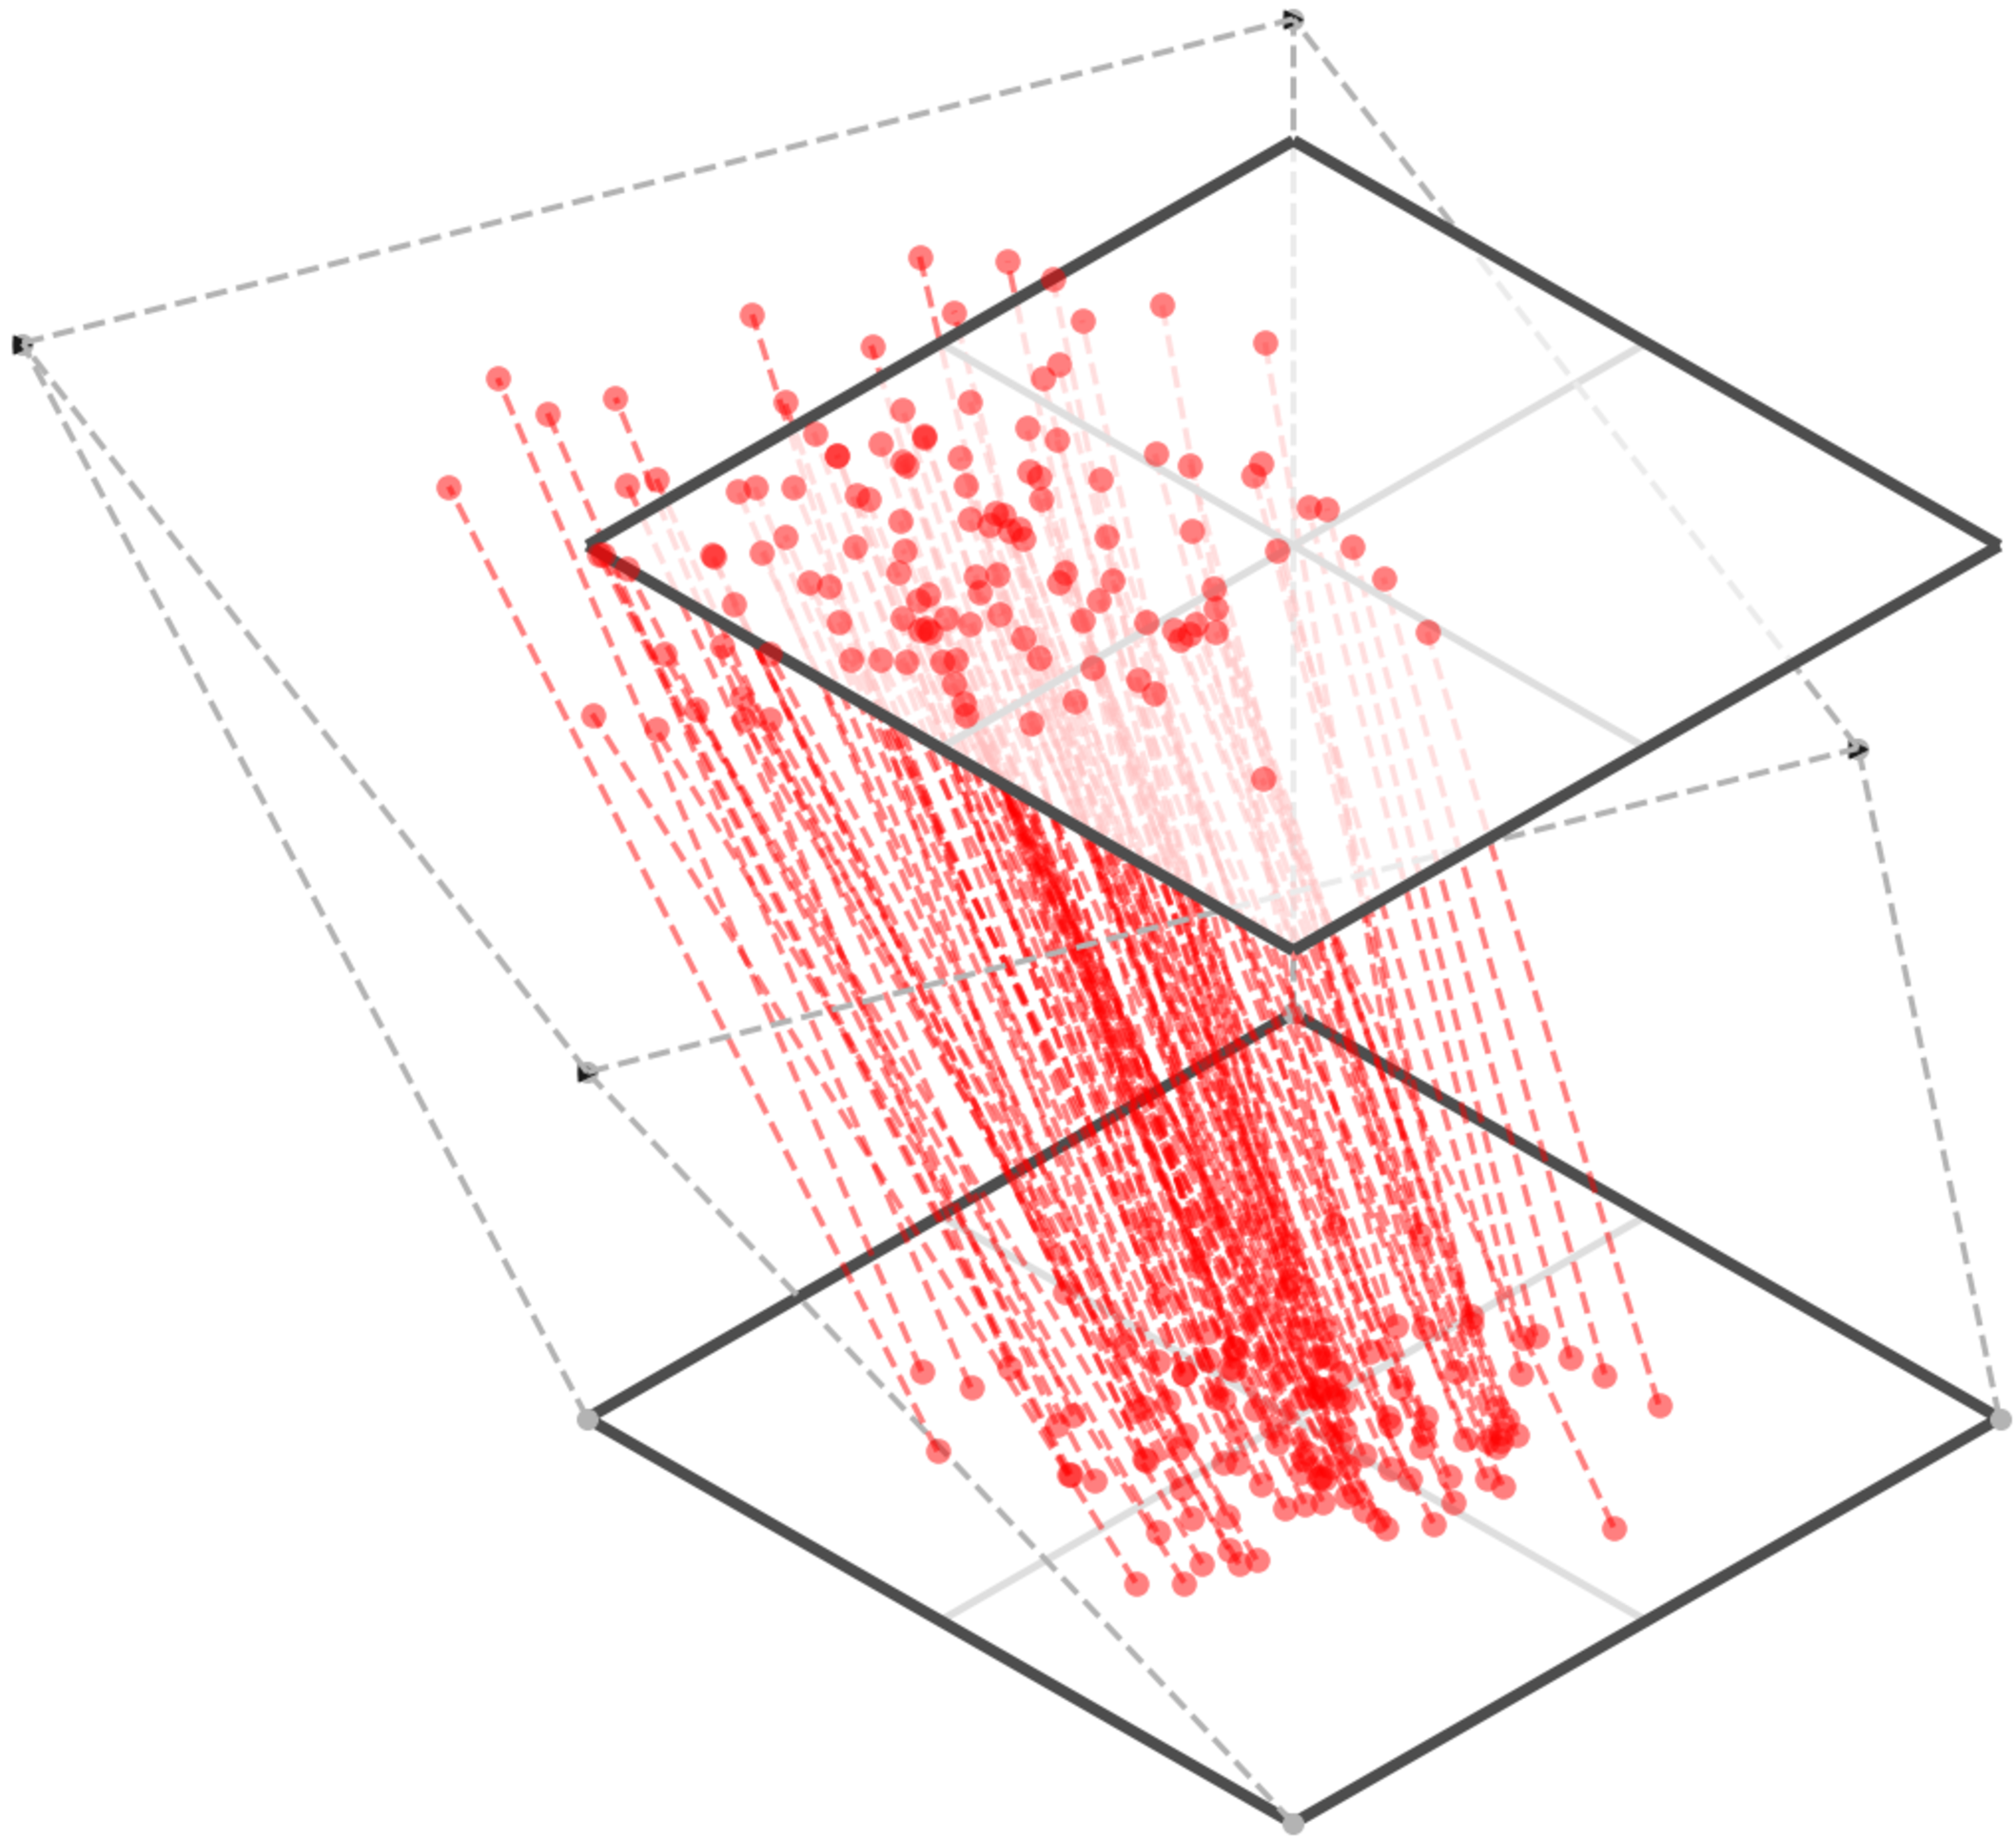
\includegraphics[width=0.8\linewidth]{figures/neural_nets/linear_layer_mapviz.pdf}};
    \draw (-1, -1.4) node {$\xin$};
    \draw (-1, 1.45) node {$\xout$};
    \draw (0, 2.3) node {\texttt{linear}};
\end{tikzpicture}
\end{minipage}
\begin{minipage}{0.28\textwidth}
\begin{tikzpicture}
    \draw (0, 0) node[inner sep=0] {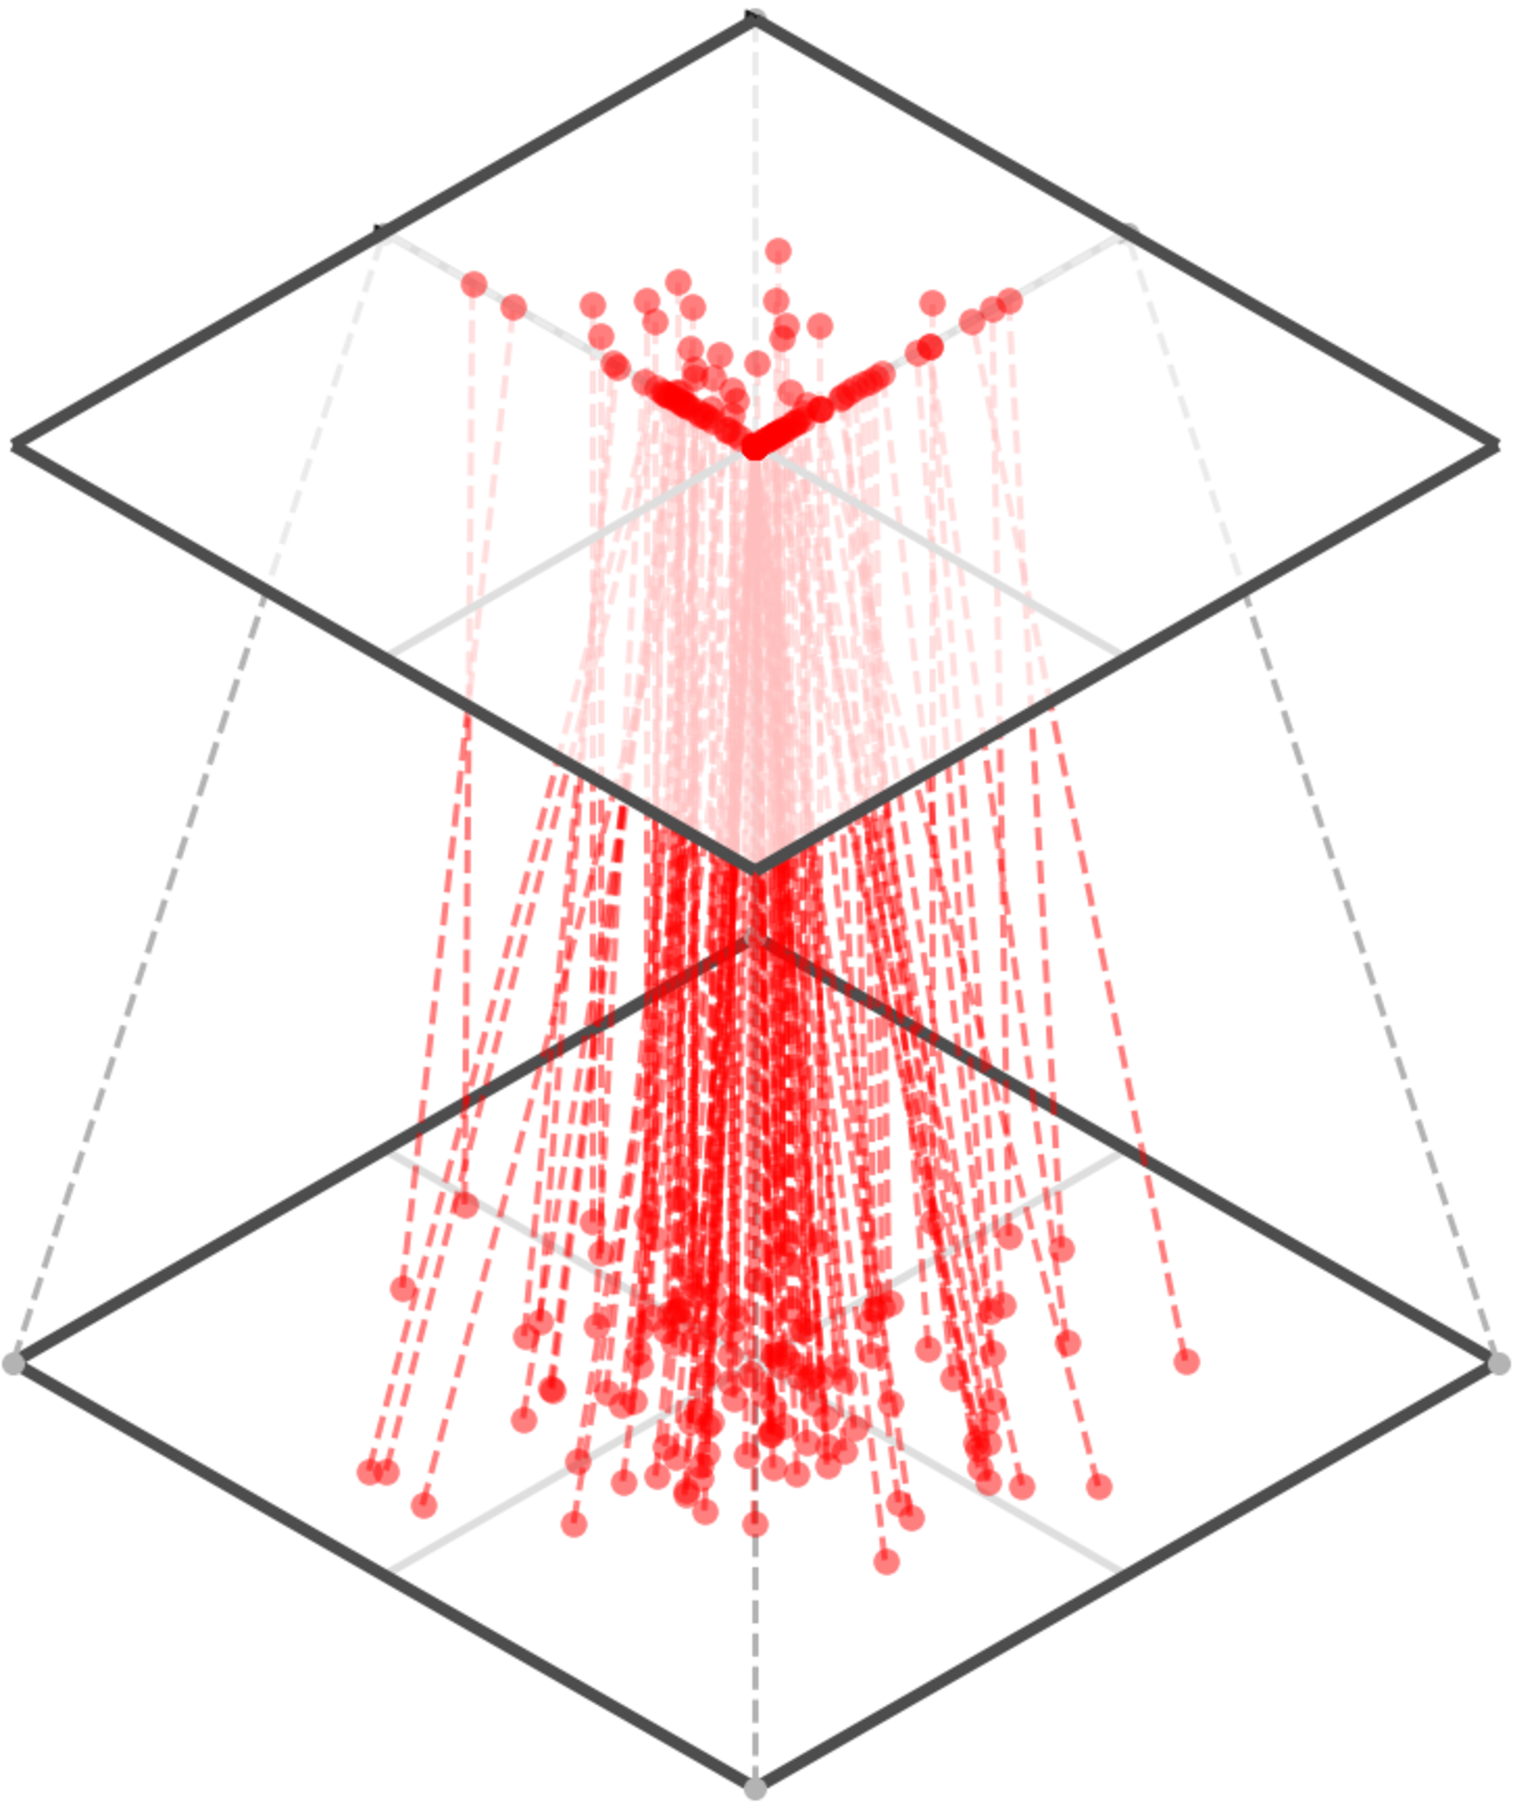
\includegraphics[width=0.8\linewidth]{figures/neural_nets/relu_layer_mapviz.pdf}};
    \draw (-1.6, -1.4) node {$\xin$};
    \draw (-1.6, 1.45) node {$\xout$};
    \draw (0, 2.3) node {\texttt{relu}};
\end{tikzpicture}
\end{minipage}
\begin{minipage}{0.28\textwidth}
\begin{tikzpicture}
    \draw (0, 0) node[inner sep=0] {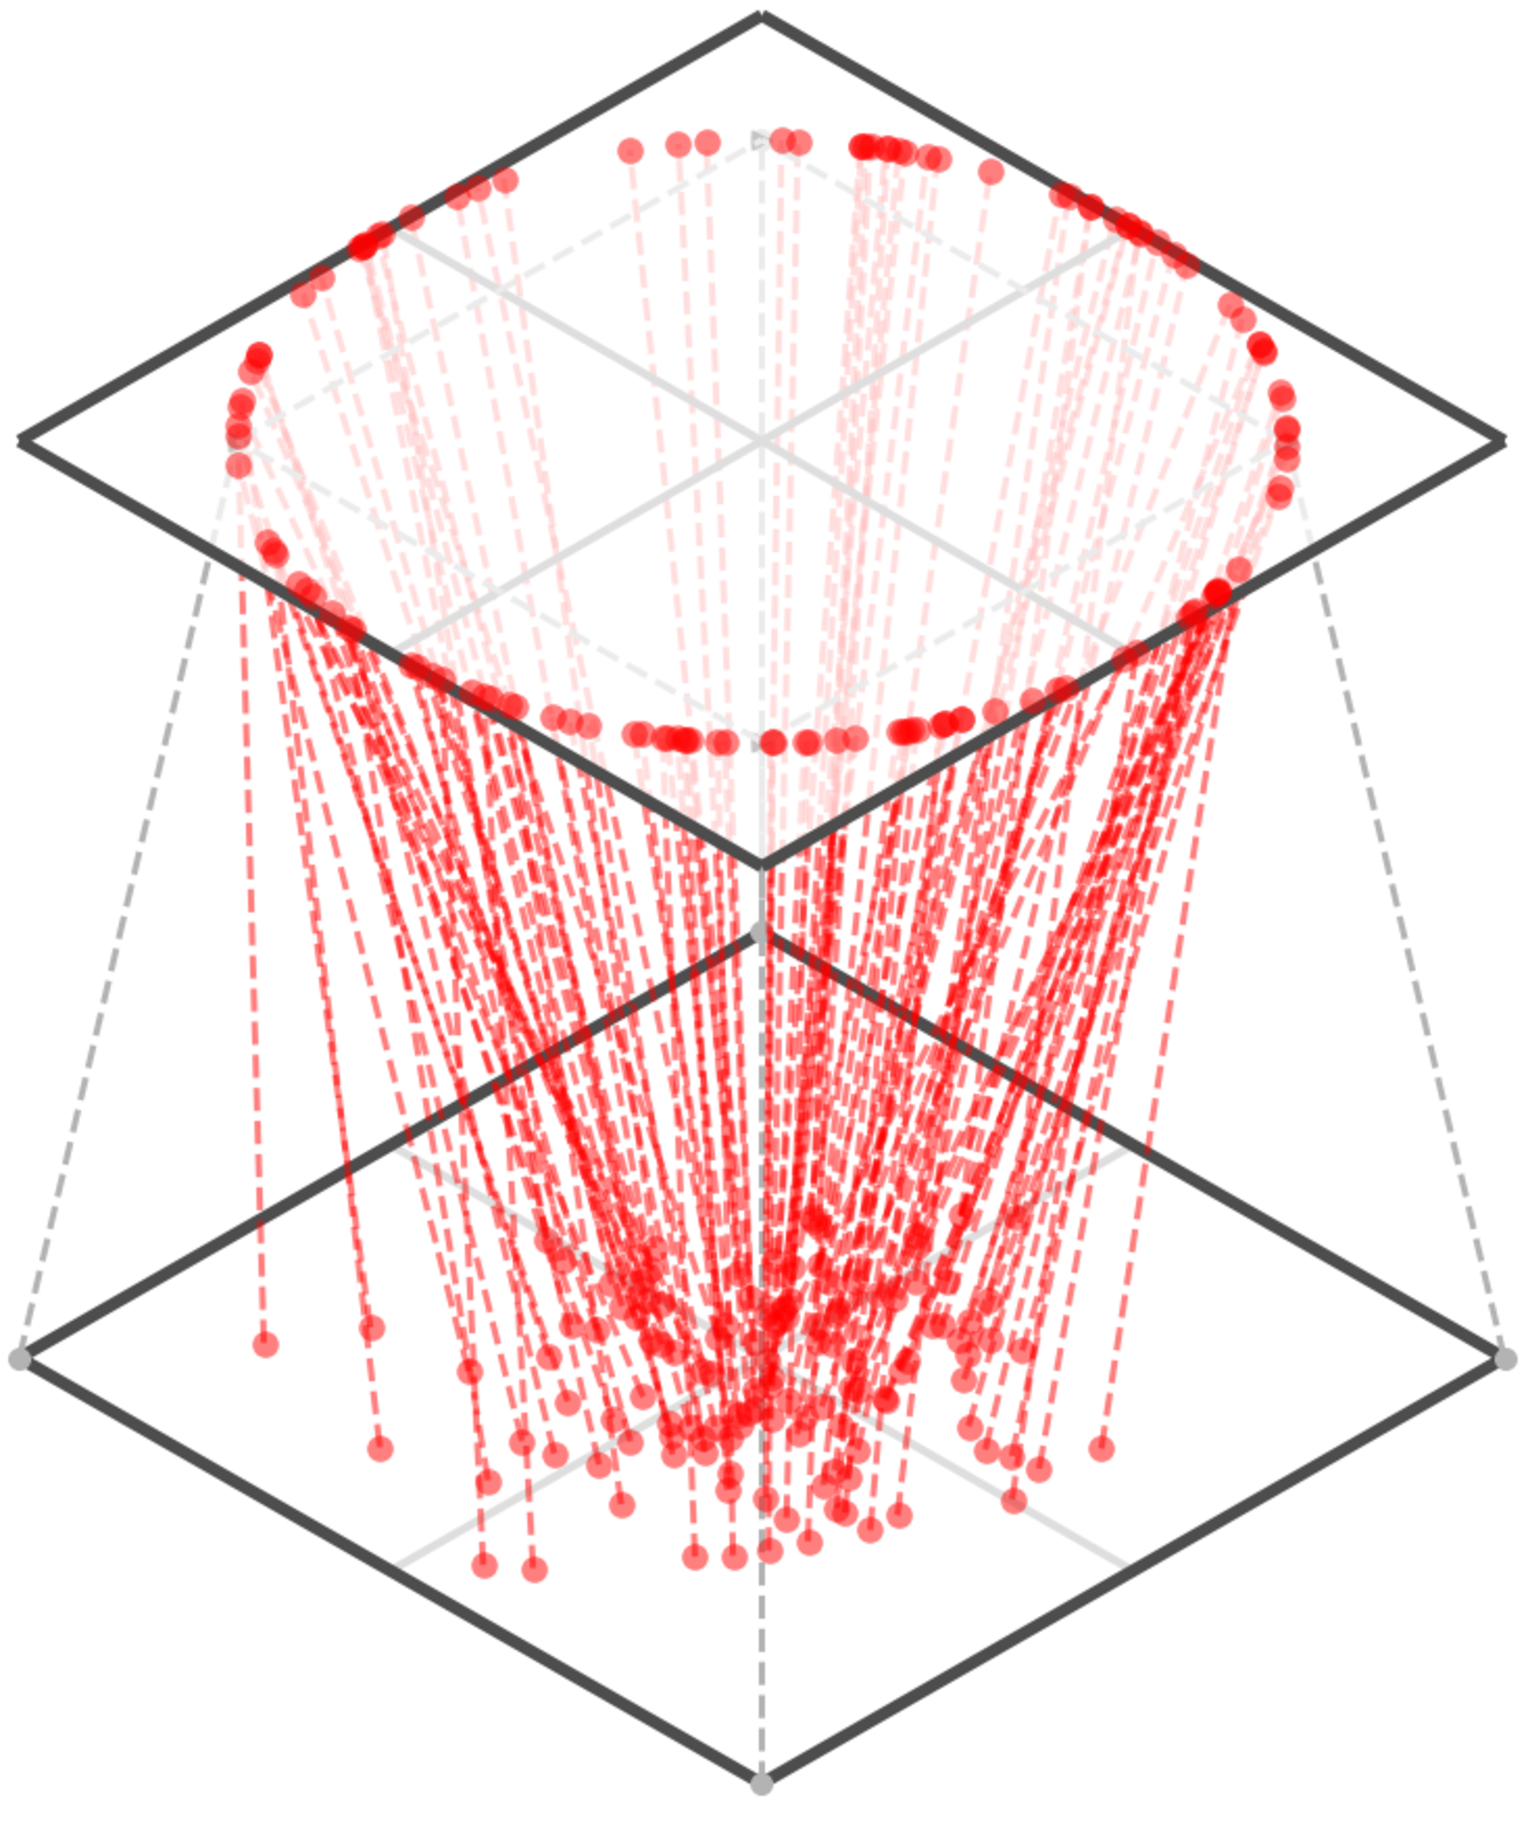
\includegraphics[width=0.8\linewidth]{figures/neural_nets/L2norm_layer_mapviz.pdf}};
    \draw (-1.6, -1.4) node {$\xin$};
    \draw (-1.6, 1.45) node {$\xout$};
    \draw (0, 2.3) node {\texttt{L2-norm}};
\end{tikzpicture}
\end{minipage}
% \begin{minipage}{0.33\textwidth}
% \begin{flushright}
% \begin{tikzpicture}
%     \draw (0, 0) node[inner sep=0] {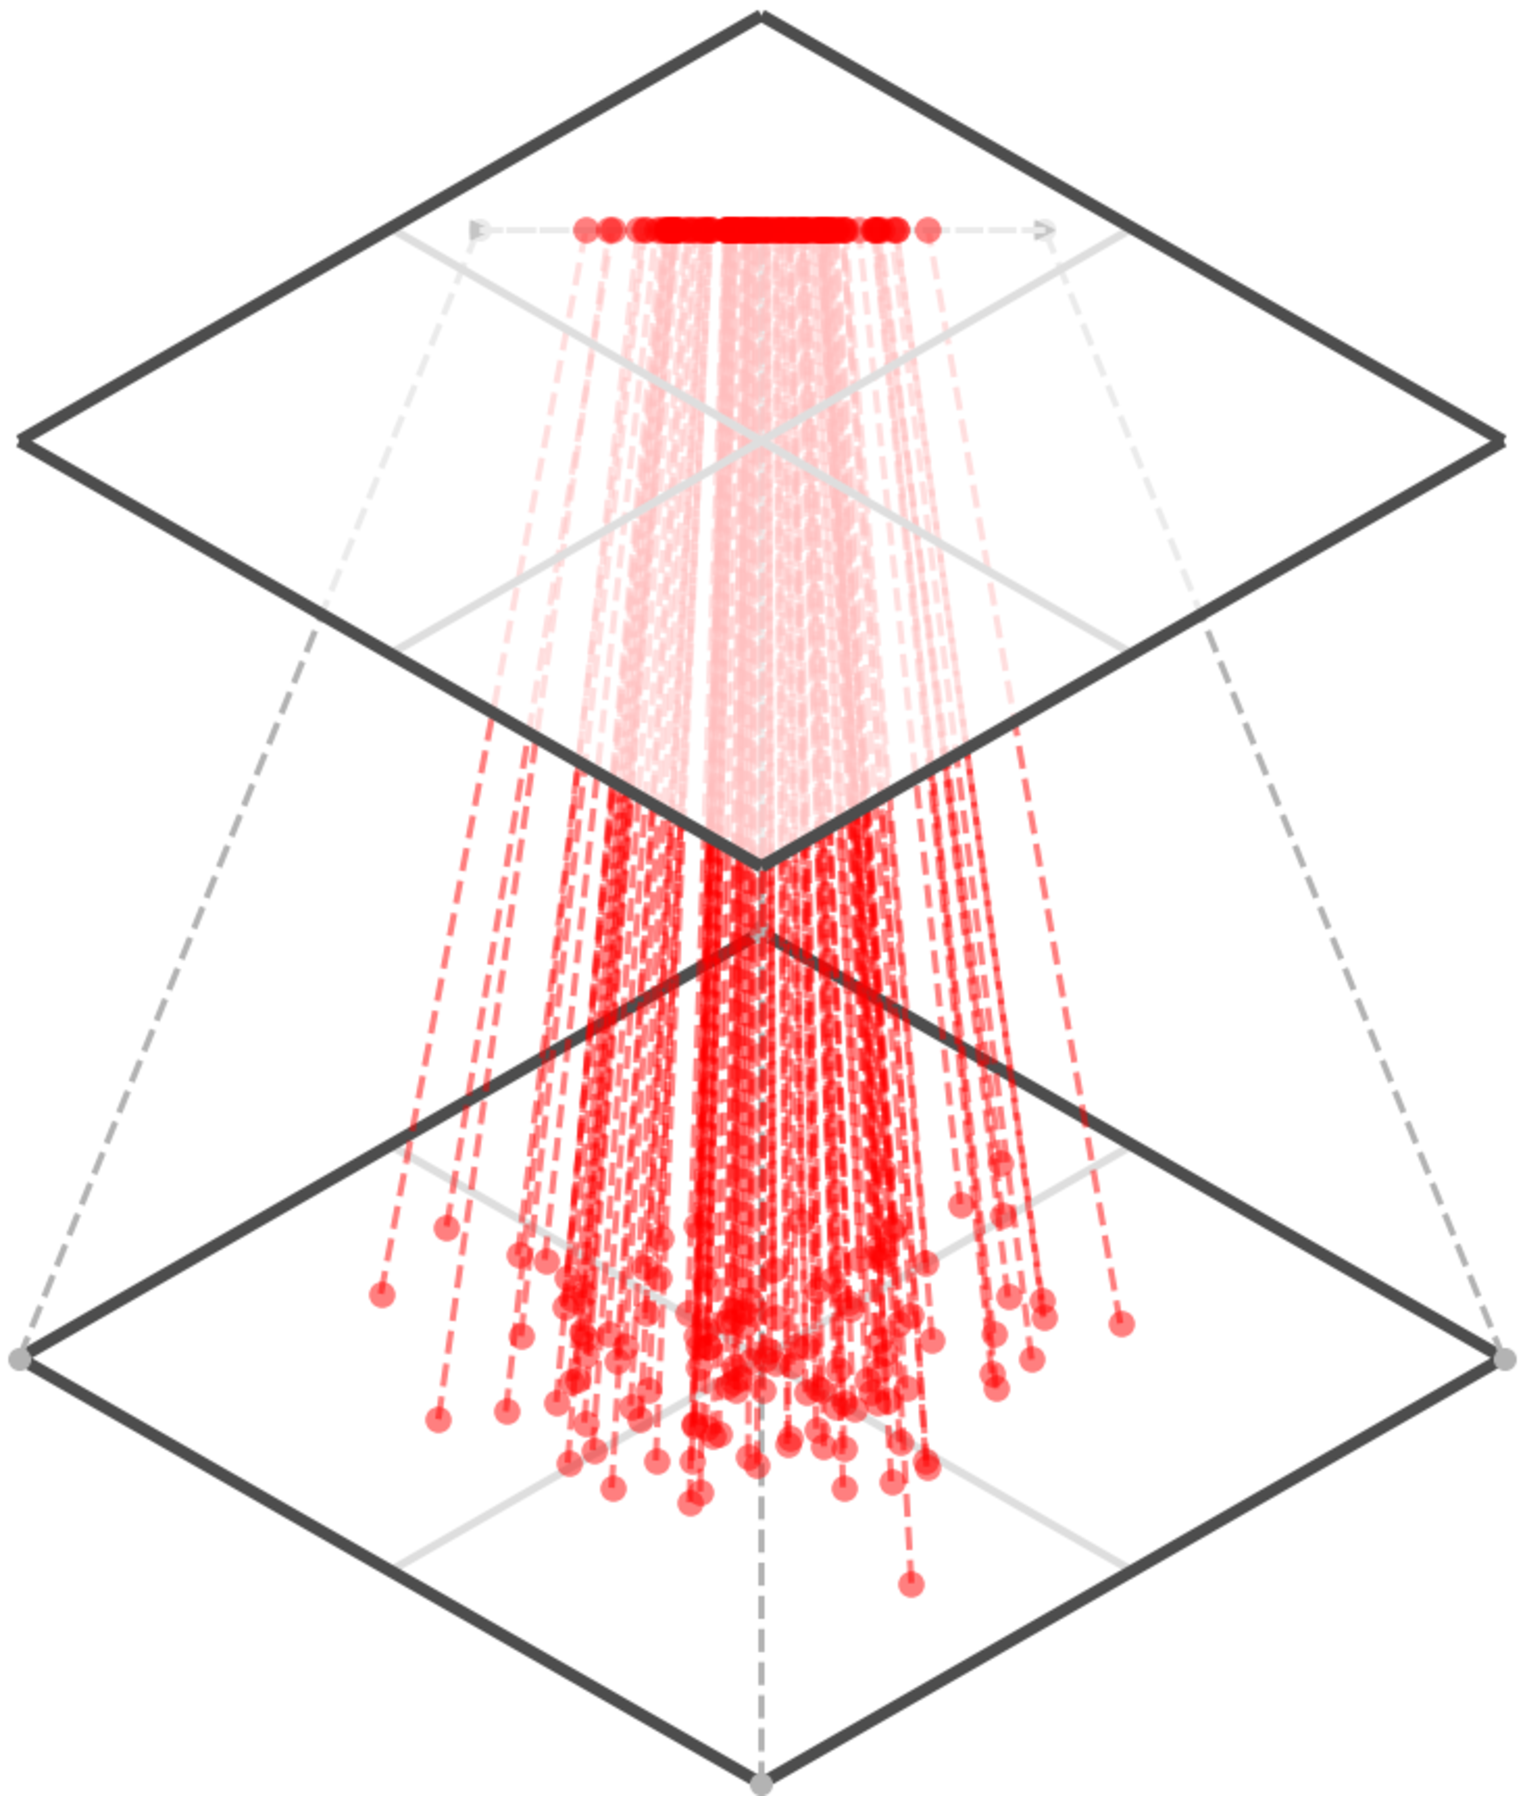
\includegraphics[width=1.0\linewidth]{figures/neural_nets/softmax_layer_mapviz.pdf}};
% \end{tikzpicture}
% \end{flushright}
% \end{minipage}
}
\caption{2D mapping diagrams for several neural layers. The \texttt{linear} layer mapping will shift, stretch, and rotate depending on its weights and biases.}
\label{fig:neural_nets_as_data_transformations:2D_mapping_diagrams}
\end{figure}


%Here is a linear layer $f: \mathbb{R}^2 \rightarrow \mathbb{R}^2$:
% Here are the linear and relu layers plotted this way, alongside other ways of representing these mappings:
% \begin{figure}[h]
%     \centerline{
%     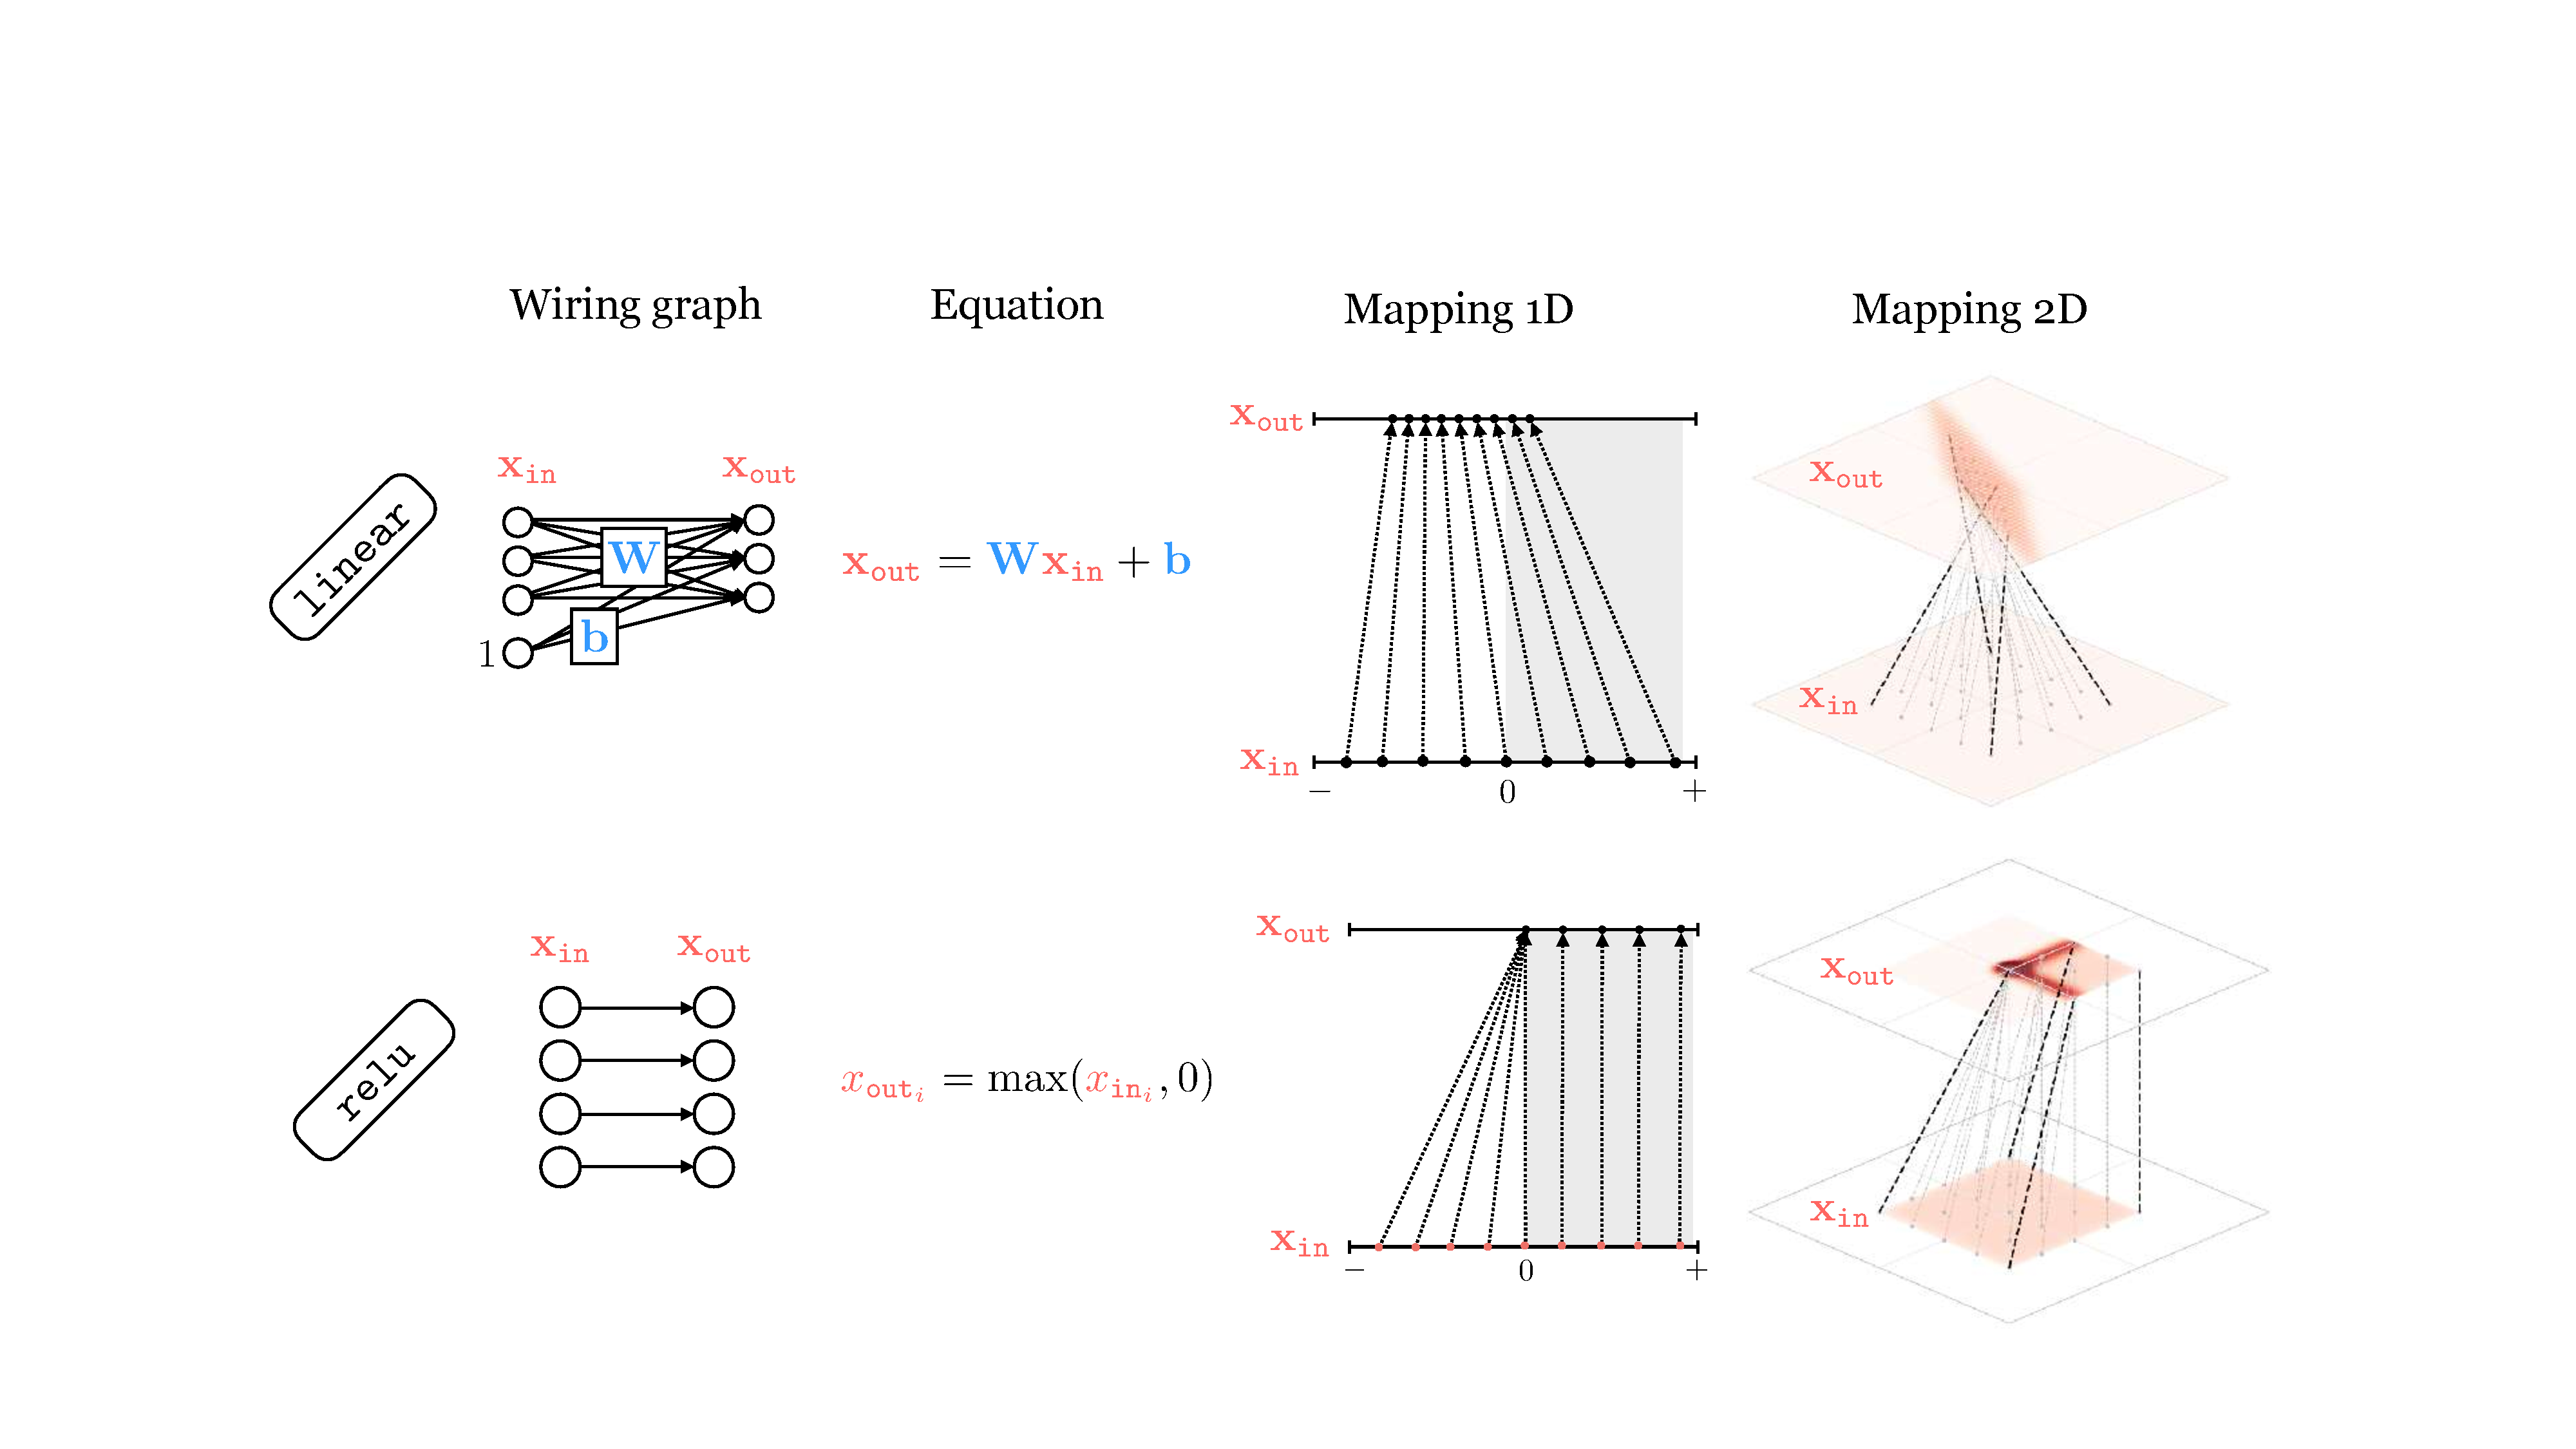
\includegraphics[width=1.0\linewidth]{./figures/neural_nets/layer_cards_linear_relu.pdf}}
%     \caption{A summary of the main two layers we have learned about so far.}
%     \label{fig:neural_nets:layer_cards_linear_relu}
% \end{figure}

One interesting thing to notice here is that the relu layer maps many points to the axes of the positive quadrant. In general, with relu-nets, a lot of data density will build up along these axes, because any point \textit{not} in the positive quadrant snaps to an axis. This effect becomes exaggerated in real networks with high-dimensional embeddings. In particular, for a width-$N$ layer, the region that is strictly positive occupies only $\frac{1}{2^N}$ proportion of the embedding space, so almost the entire space gets mapped to the axes after a relu layer. The geometry of high-dimensional neural representations may become very sparse because of this, where most of the volume of representational space is not occupied by any datapoints.
%This is because relu snaps all negative coordinates to zero, so any point in the negative subspace will end up mapping to an ``edge" of the positive quadrant.

% \begin{figure}[h]
%     \centering
%     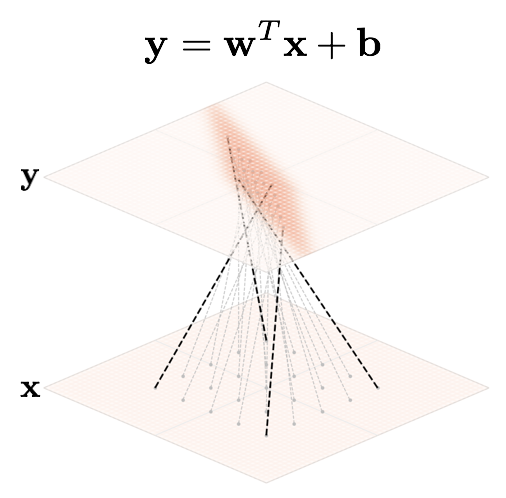
\includegraphics[width=0.36\linewidth]{./figures/neural_nets_as_data_transformations/2D_linear_layer.png}
%     \label{fig:neural_nets_as_data_transformations:2D_linear_layer}
% \end{figure}

%The data can be thought of as itself a representation. The target output, e.g., class labels, is another representation. Then a classifier network, layer by layer, maps a representations that matches the raw data to a representation that matches the labels. The sequence of representations for an input datapoint $\xin^i$ is $\xin^i \rightarrow \mathbf{h}^{(1)i} \rightarrow \mathbf{h}^{(2)i} \rightarrow \cdots \rightarrow \xout^i$.

%One way to characterize this sequence of representations is by looking at how each subsequent layer represents an entire \emph{dataset}. 


\section{Binary Classifier Example}
Consider a multilayer perceptron (MLP) that performs binary classification formulated as two-way softmax regression. The input datapoints are each in $\mathbb{R}^2$ and the target outputs are in $\vartriangle^1$ (the one-simplex), %\marginnote{The {\bf N-simplex}, $\vartriangle^N$, is the set of all $N+1$ dimensional vectors whose elements sum to 1. $N+1$ dim one-hot codes live on the vertices of $\vartriangle^{N}$.}[-1.0cm] 
with layer structure $\texttt{linear}-\texttt{relu}-\texttt{linear}-\texttt{relu}-\texttt{linear}$. This network is drawn below in \fig{\ref{fig:neural_nets:simple_MLP_network2}}:

\begin{figure}[h]
\centerline{

%\noindent\hspace{0.05\linewidth}
%\begin{minipage}{.45\linewidth}

\begin{tikzpicture}[>=spaced latex]
% linear1
\draw [thick] (0,-0.4) circle [radius=0.3] node {$x_2$};
\draw [thick] (0,0.4) circle [radius=0.3] node {$x_1$};
\draw [thick] [nn_edge] (0.3,-0.4) -- (1.0,-0.4);
\draw [thick] [nn_edge] (0.3,0.4) -- (1.0,0.4);
\draw [thick] [nn_edge] (0.3,-0.4) -- (1.0,0.4);
\draw [thick] [nn_edge] (0.3,0.4) -- (1.0,-0.4);
\draw [thick, fill=gray_neuron] (1.3,-0.4) circle [radius=0.3] node {$z_{1_1}$};
\draw [thick, fill=gray_neuron] (1.3,0.4) circle [radius=0.3] node {$z_{1_2}$};
\draw [thick,dotted] (0.5,-0.9)  .. controls (0.6,-0.75) .. (0.6,-0.6);
\draw (0.6,-1.2) node {$\mathbf{W}_1$};

% relu1
\draw [thick] [nn_edge] (1.6,-0.4) -- (2.3,-0.4);
\draw [thick] [nn_edge] (1.6,0.4) -- (2.3,0.4);
\draw [thick, fill=gray_neuron] (2.6,-0.4) circle [radius=0.3] node {$h_{1_1}$};
\draw [thick, fill=gray_neuron] (2.6,0.4) circle [radius=0.3] node {$h_{1_2}$};

% linear2
\draw [thick] [nn_edge] (2.9,-0.4) -- (3.6,0.4);
\draw [thick] [nn_edge] (2.9,0.4) -- (3.6,-0.4);
\draw [thick] [nn_edge] (2.9,-0.4) -- (3.6,-0.4);
\draw [thick] [nn_edge] (2.9,0.4) -- (3.6,0.4);
\draw [thick, fill=gray_neuron] (3.9,-0.4) circle [radius=0.3] node {$z_{2_1}$};
\draw [thick, fill=gray_neuron] (3.9,0.4) circle [radius=0.3] node {$z_{2_2}$};
\draw [thick,dotted] (3.2,-0.9)  .. controls (3.3,-0.75) .. (3.3,-0.6);
\draw (3.3,-1.2) node {$\mathbf{W}_2$};

% relu2
\draw [thick] [nn_edge] (4.2,-0.4) -- (4.9,-0.4);
\draw [thick] [nn_edge] (4.2,0.4) -- (4.9,0.4);
\draw [thick, fill=gray_neuron] (5.2,-0.4) circle [radius=0.3] node {$h_{1_1}$};
\draw [thick, fill=gray_neuron] (5.2,0.4) circle [radius=0.3] node {$h_{1_2}$};

% linear3
\draw [thick] [nn_edge] (5.5,-0.4) -- (6.2,0.4);
\draw [thick] [nn_edge] (5.5,0.4) -- (6.2,-0.4);
\draw [thick] [nn_edge] (5.5,-0.4) -- (6.2,-0.4);
\draw [thick] [nn_edge] (5.5,0.4) -- (6.2,0.4);
\draw [thick, fill=gray_neuron] (6.5,-0.4) circle [radius=0.3] node {$z_{2_1}$};
\draw [thick, fill=gray_neuron] (6.5,0.4) circle [radius=0.3] node {$z_{2_2}$};
\draw [thick,dotted] (5.8,-0.9)  .. controls (5.9,-0.75) .. (5.9,-0.6);
\draw (5.9,-1.2) node {$\mathbf{W}_3$};

% softmax
\draw [thick] [nn_edge] (6.8,-0.4) -- (7.5,-0.4);
\draw [thick] [nn_edge] (6.8,0.4) -- (7.5,0.4);
\draw [thick] (7.8,-0.4) circle [radius=0.3] node {$y_1$};
\draw [thick] (7.8,0.4) circle [radius=0.3] node {$y_2$};
\end{tikzpicture}
%\end{minipage}
}
\caption{An MLP with three linear layers and two outputs, suitable for performing binary softmax regression.}
%\vspace{-1.0cm}
\label{fig:neural_nets:simple_MLP_network2}
\end{figure}

Or expressed in math as follows:
\begin{align}
    \mathbf{z}_1 &= \mathbf{W}_1\mathbf{x} + \mathbf{b}_1 &\triangleleft \quad \texttt{linear}\\
    \mathbf{h}_1 &= \texttt{relu}(\mathbf{z}_1) &\triangleleft \quad \texttt{relu}\\
    \mathbf{z}_2 &= \mathbf{W}_2\mathbf{h}_1 + \mathbf{b}_2 &\triangleleft \quad \texttt{linear}\\
    \mathbf{h}_2 &= \texttt{relu}(\mathbf{z}_2) &\triangleleft \quad \texttt{relu}\\
    \mathbf{z}_3 &= \mathbf{W}_3\mathbf{h}_2 + \mathbf{b}_3 &\triangleleft \quad \texttt{linear}\\
    \mathbf{y} &= \texttt{softmax}(\mathbf{z}_3) &\triangleleft \quad \text{\texttt{softmax}}
\end{align}

% Or in Pytorch-like pseudocode as:
% \begin{figure}[h]
% %\centerline{
% \begin{minipage}{0.5\linewidth}
% \begin{minted}[
% fontsize=\fontsize{8.5}{9},
% frame=single,
% framesep=2.5pt,
% baselinestretch=1.05,
% ]{python}
% # W1, b1, W2, b2 : parameters of the net
% # X : dataset to run through net

% # first define parameterized layers
% fc1 = nn.linear(W1, b1)
% fc2 = nn.linear(W2, b2)

% # then run data through network
% for x in X:
%     z1 = fc1(x)
%     h1 = nn.relu(z1)
%     z2 = fc2(h1)
%     y = nn.softmax(z2)
% \end{minted}
% \end{minipage}
% \cation{Pytorch-like pseudocode for the MLP in Figure \ref{fig:neural_nets:simple_MLP_network2}.}
% %}
% \end{figure}

Now we wish to train this net to classify between two data distributions. The goal is to transform the input distribution into a target distribution that separates the classes, as shown in \fig{\ref{fig:neural_nets_as_data_transformations:goal_of_classifier}}.
\begin{figure}[h]
    \centerline{
    \begin{minipage}{0.28\textwidth}
    \begin{tikzpicture}
        \draw (0, 0) node[inner sep=0] {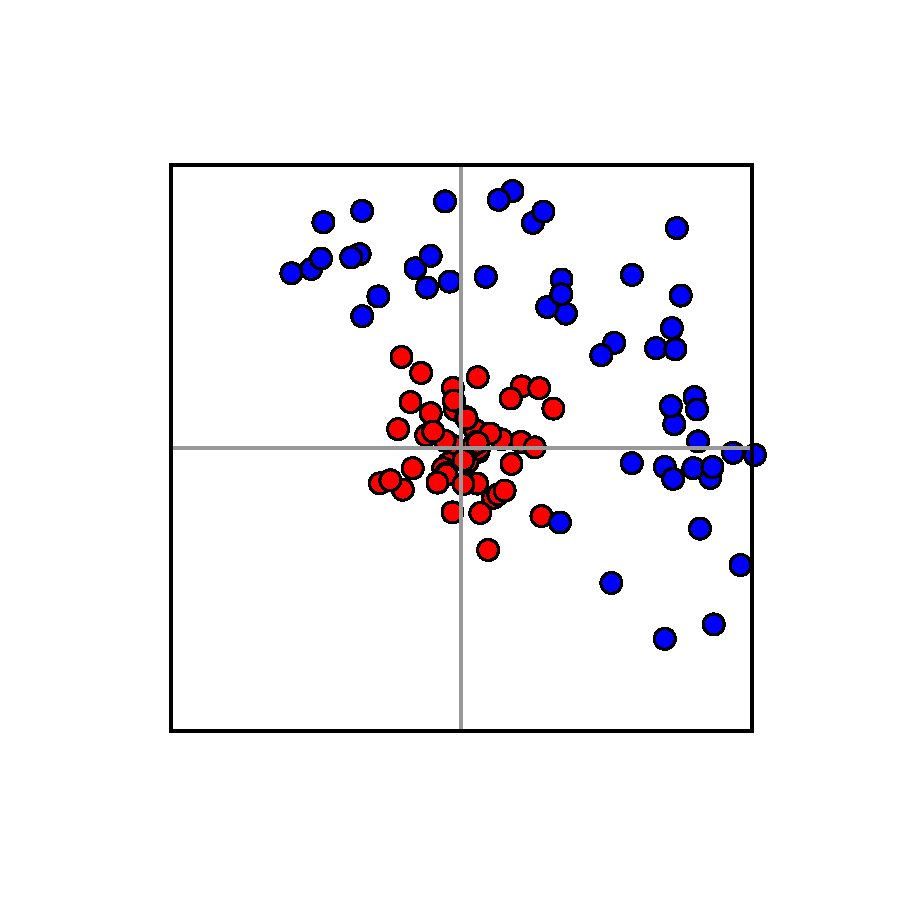
\includegraphics[width=0.75\linewidth]{figures/neural_nets/binary_classifier_example_training_data2.pdf}};
        \draw (-1.2, 1.2) node {$\mathbf{x}$};
        \draw (0, 1.75) node {Input data};
        %
        
        % neural net mapping
        \draw [thick,->] (2, 0) -- (6.5, 0);
        \def\Nlayers{6}
        \def\layerheight{0.6}
        \def\layerstep{0.3}
        \foreach \x in {1,...,\Nlayers} {
            \draw [fill=white] (\layerstep*\x+3.1,-\layerheight/2) rectangle ++(\layerheight/4,\layerheight);
        }
        %\draw (4.25, 0) node[fill=white] {$?$};
        \draw (4.25, 0.75) node {Series of geometric transformations};
        \draw (4.25, -0.75) node {(i.e., a neural net)};
        %
    \end{tikzpicture}
    \end{minipage}
    \begin{minipage}{0.28\textwidth}
    \begin{tikzpicture}
        %\draw (0, 1) node {$?$};
        %\draw [thick,->] (0, 1) -- (1, 1);
    \end{tikzpicture}
    \end{minipage}
    \begin{minipage}{0.28\textwidth}
    \begin{tikzpicture}
        \draw (0, 0) node[inner sep=0] {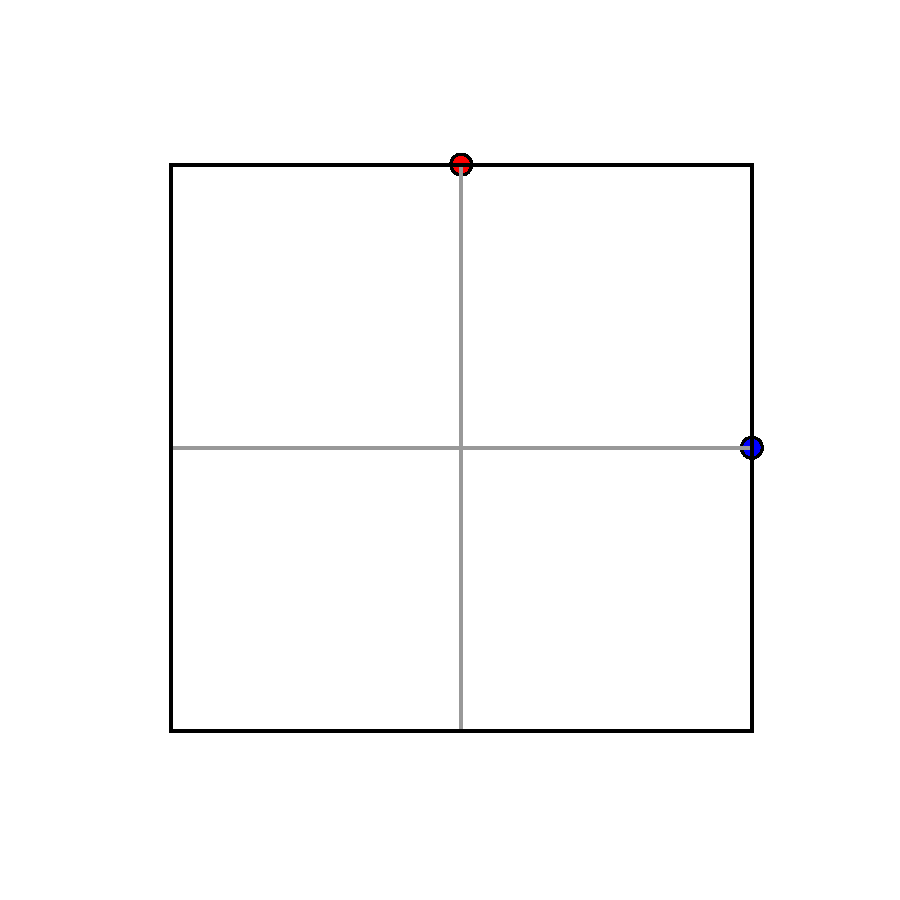
\includegraphics[width=0.75\linewidth]{figures/neural_nets/binary_classifier_ex_targets.pdf}};
        \draw (-1.2, 1.2) node {$\mathbf{y}$};
        \draw (0, 1.75) node {Target output};
    \end{tikzpicture}
    \end{minipage}
    }
    \caption{The goal of a neural net classifier is to rearrange the input data distribution to match the target label distribution. (left) Input dataset with two classes in red and blue. (right) Target output (one-hot codes).}
    \label{fig:neural_nets_as_data_transformations:goal_of_classifier}
\end{figure}

In this example, the target output places all the red dots at $(0,1)$ and all the blue dots at $(1,0)$. These are the coordinates of one-hot codes for our two classes. Training the network consists of find the series of geometric transformations that rearrange the input distribution to this target output distribution.

We will visualize how the net transforms the training dataset, layer by layer, at four \index{Checkpoint}{\bf checkpoints} over the course of training.\marginnote{A checkpoint is a record of the parameters at some iteration of training, that is, if iterates of the parameter vector are $\theta^0, \theta^1, \ldots, \theta^T$, then any $\theta^k$ can be recorded as a checkpoint.}[-2.2cm] In \fig{\ref{fig:neural_nets:nn_training_viz}}, we plot this as a 3D visualization of $\mathbb{R}^2 \rightarrow \mathbb{R}^2$ mappings. Each dotted line connects the representation of a datapoint at one layer to its representation at the next. The gray lines show, for each layer, how a square region around the origin gets stretched, rotated, or squished to map to a transformed region on the next layer.
\begin{figure}[h]
    \centerline{
    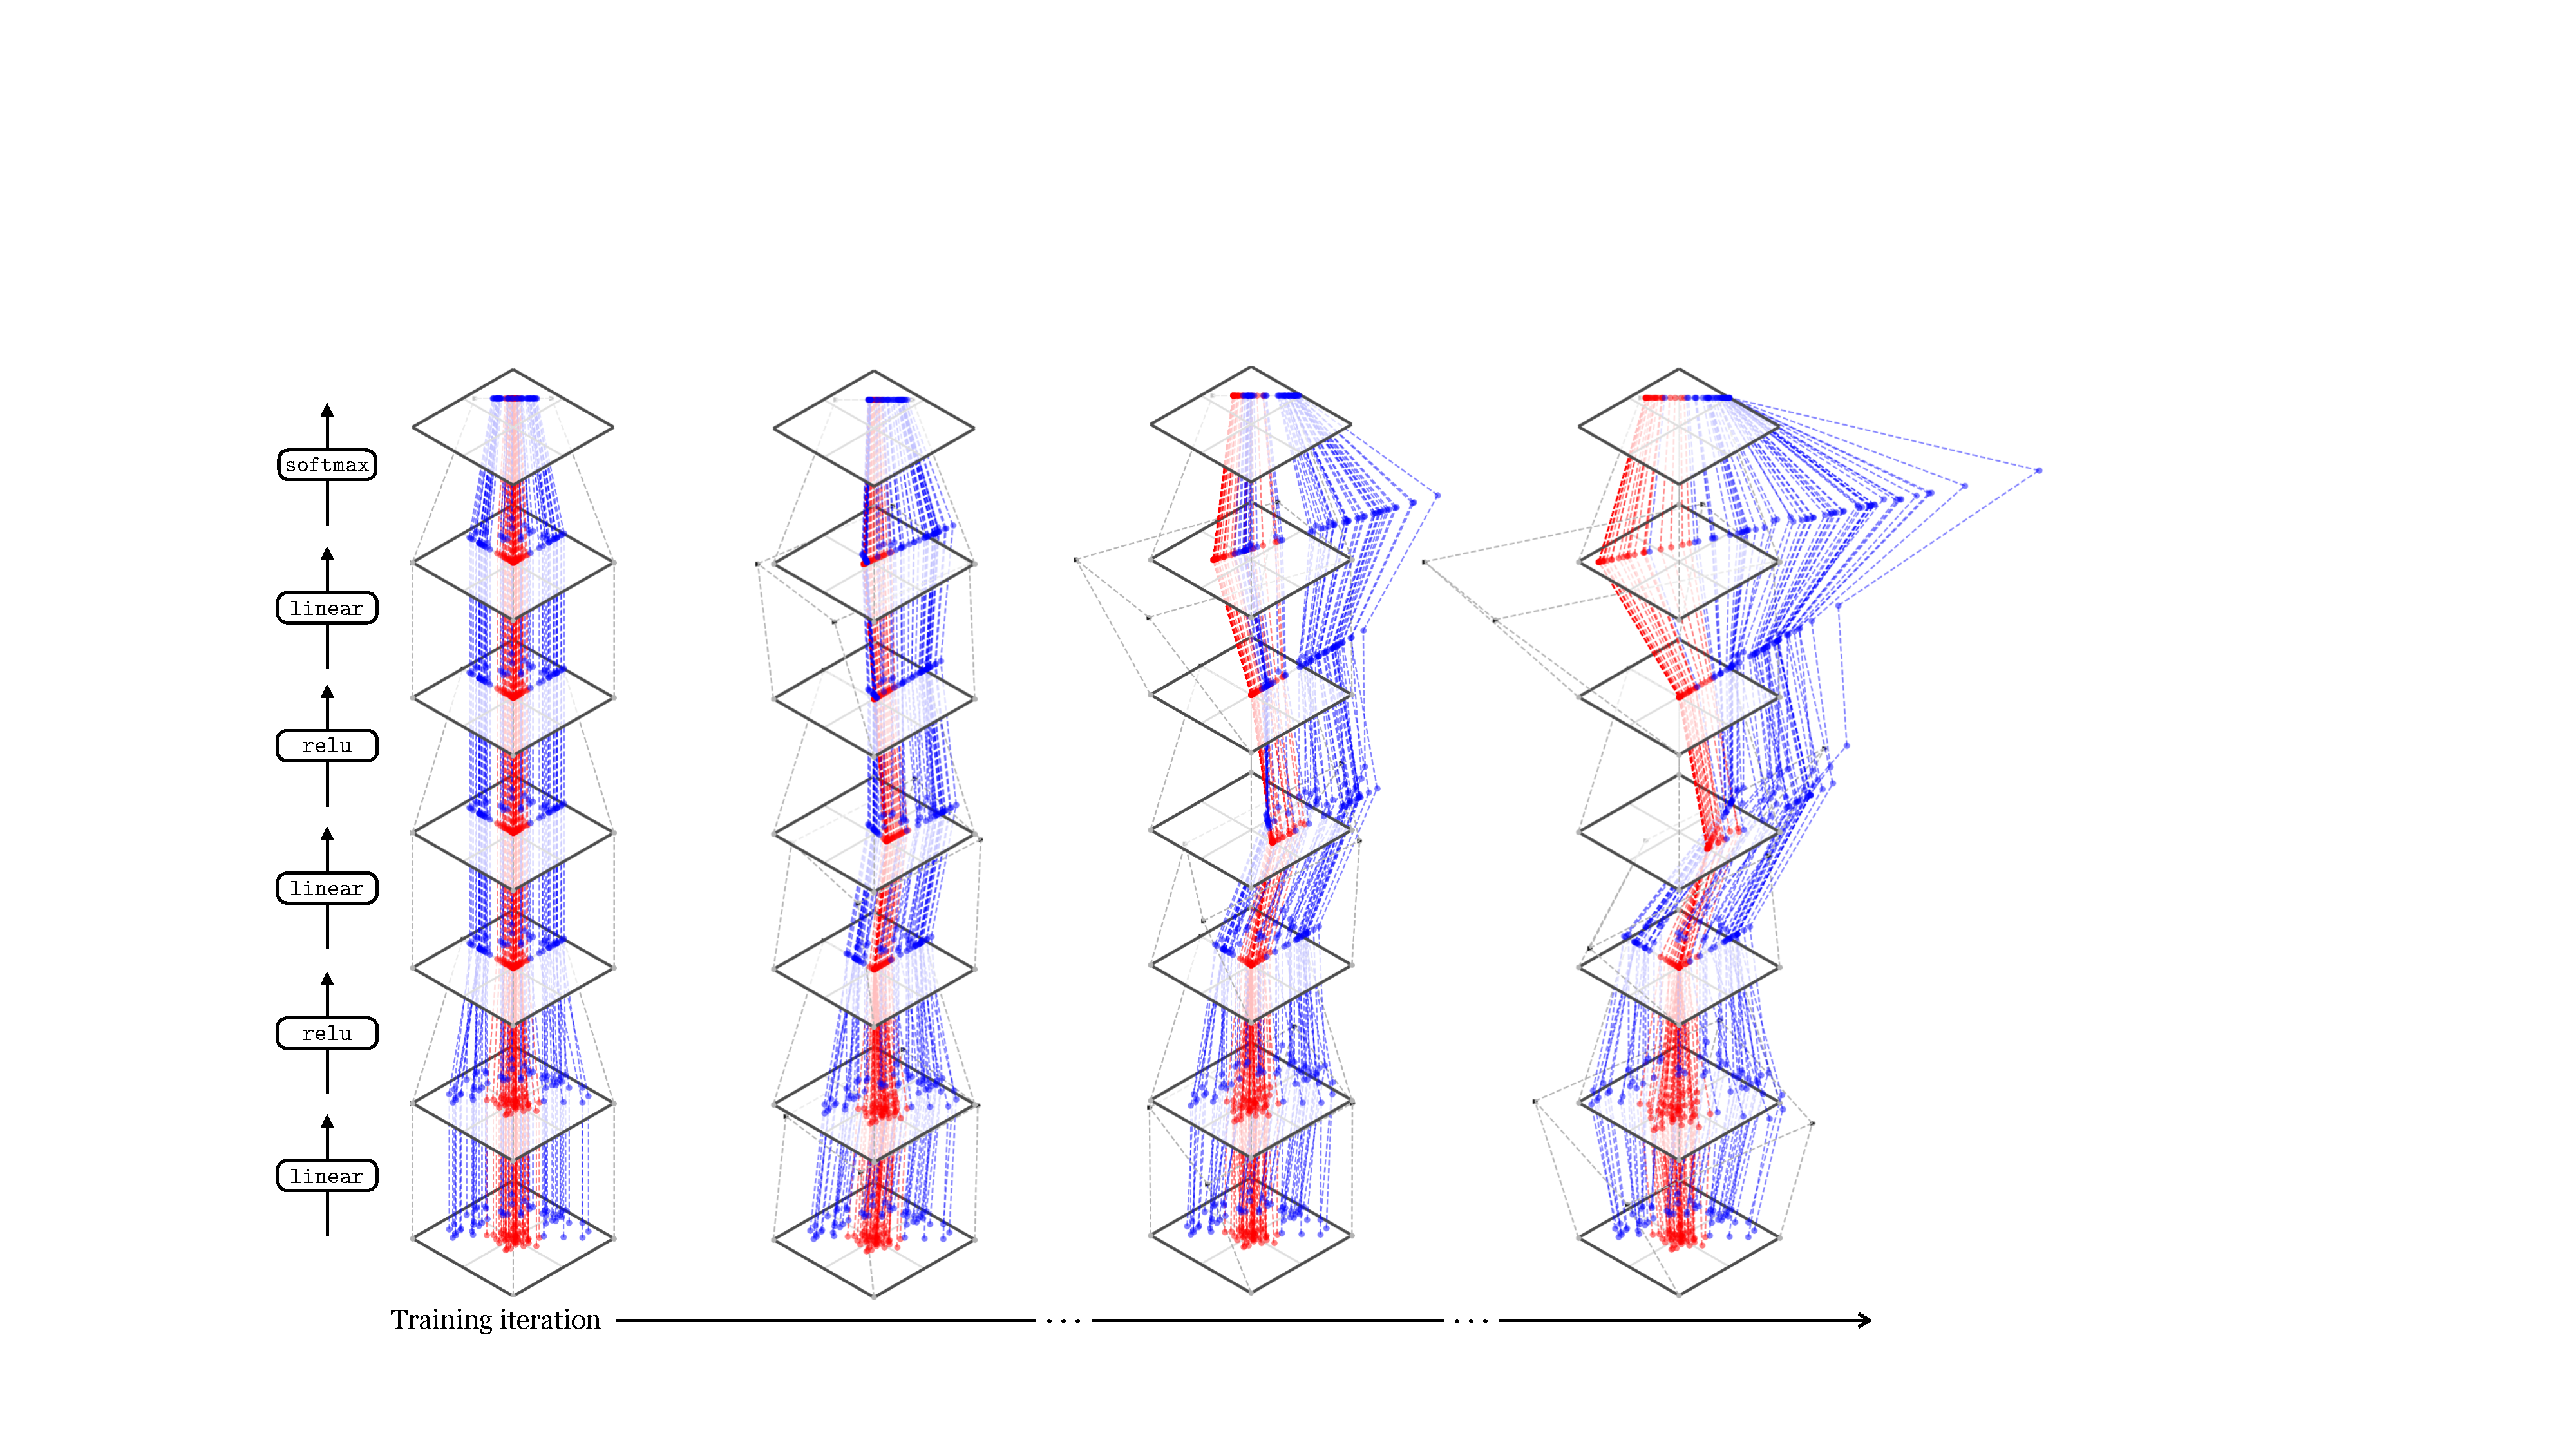
\includegraphics[width=1.0\linewidth]{./figures/neural_nets/nn_training_viz2.pdf}
    }
    \caption{How a deep net remaps input data layer by layer. The target output is to move all the red points to $(0,1)$ and all the blue points to $(1,0)$ (one-hot codes for the two classes). As training progresses the network gradually achieves this separation.}
    \label{fig:neural_nets:nn_training_viz}
\end{figure}

Of course, ``stretched, rotated, or squished'' is just an intuitive way to think about it, but we can be more precise. The linear layers perform an affine transformation of the space, while the relus project all negative values to the boundaries of the cone whose dimensions are strictly positive. Layer by layer, over the course of training, the net learns to disentangle these two classes and pull the points toward vertices of the one-simplex, achieving a correct classification of the points!


\section{How High-Dimensional Datapoints Get Remapped by Deep Net}
%When the represntation $\mathbf{h}^{(1)i}$ were a two-dimensional vector, then we could visualize this representation for all datapoints $i$ in a dataset as a 2D scatter plot. If the next layer $\mathbf{h}^{(2)i}$ were also two-dimensional, then it would be a different scatter plot, with each datapoint shifted to a new position. Typically, each hidden layer is a high-dimensional vector, so it's non-trivial to visualize datapoints in this space.
What if our data and activations are high-dimensional? The plots above only can visualize 1D and 2D data distributions. Deep representations are typically much higher-dimensional than this, and to visualize them, we need to apply tools from {\bf dimensionality reduction}. These tools project the high-dimensional data to a lower dimensionality, for example 2D, which can be visualized. A common objective is to perform the projection such that the distance between two datapoints in the 2D projection is roughly proportional to their actual distance in the high-dimensional space. In the next plot, \fig{\ref{fig:neural_nets:vit_mapping_plot}}, we use a dimensionality reduction technique called \textbf{t-Distributed Stochastic Neighbor Embedding} \textbf{t-SNE}~\cite{tsne} to visualize how different layers of a modern deep net represent a dataset of images of different semantic classes, where each color represents a different semantic class. The network we are visualizing is of the transformer architecture, and we will learn about all its details in \chap{\ref{chapter:transformers}}. For now, the important things to note are that (1) we are only showing a selected few of the layers (this net actually has dozen of layers) and (2) the embeddings are high-dimensional (in particular, they are 38,400-dimensional) but mapped down to 2D by t-SNE. Therefore, this visualization is just a rough view of what is going on in the net, unlike the visualizations in the previous section, which showed the exact embeddings and every single step of the layer-to-layer transformations.
%The following plot uses a dimensionality reduction technique called t-SNE~\cite{tsne} to visualize how different layers of a deep net represent a dataset of images of different semantic classes, where each color represents a different semantic class:
%The following plot, reproduced from \cite{decaf}, 
% \begin{figure}[h]
%     \centerline{
%     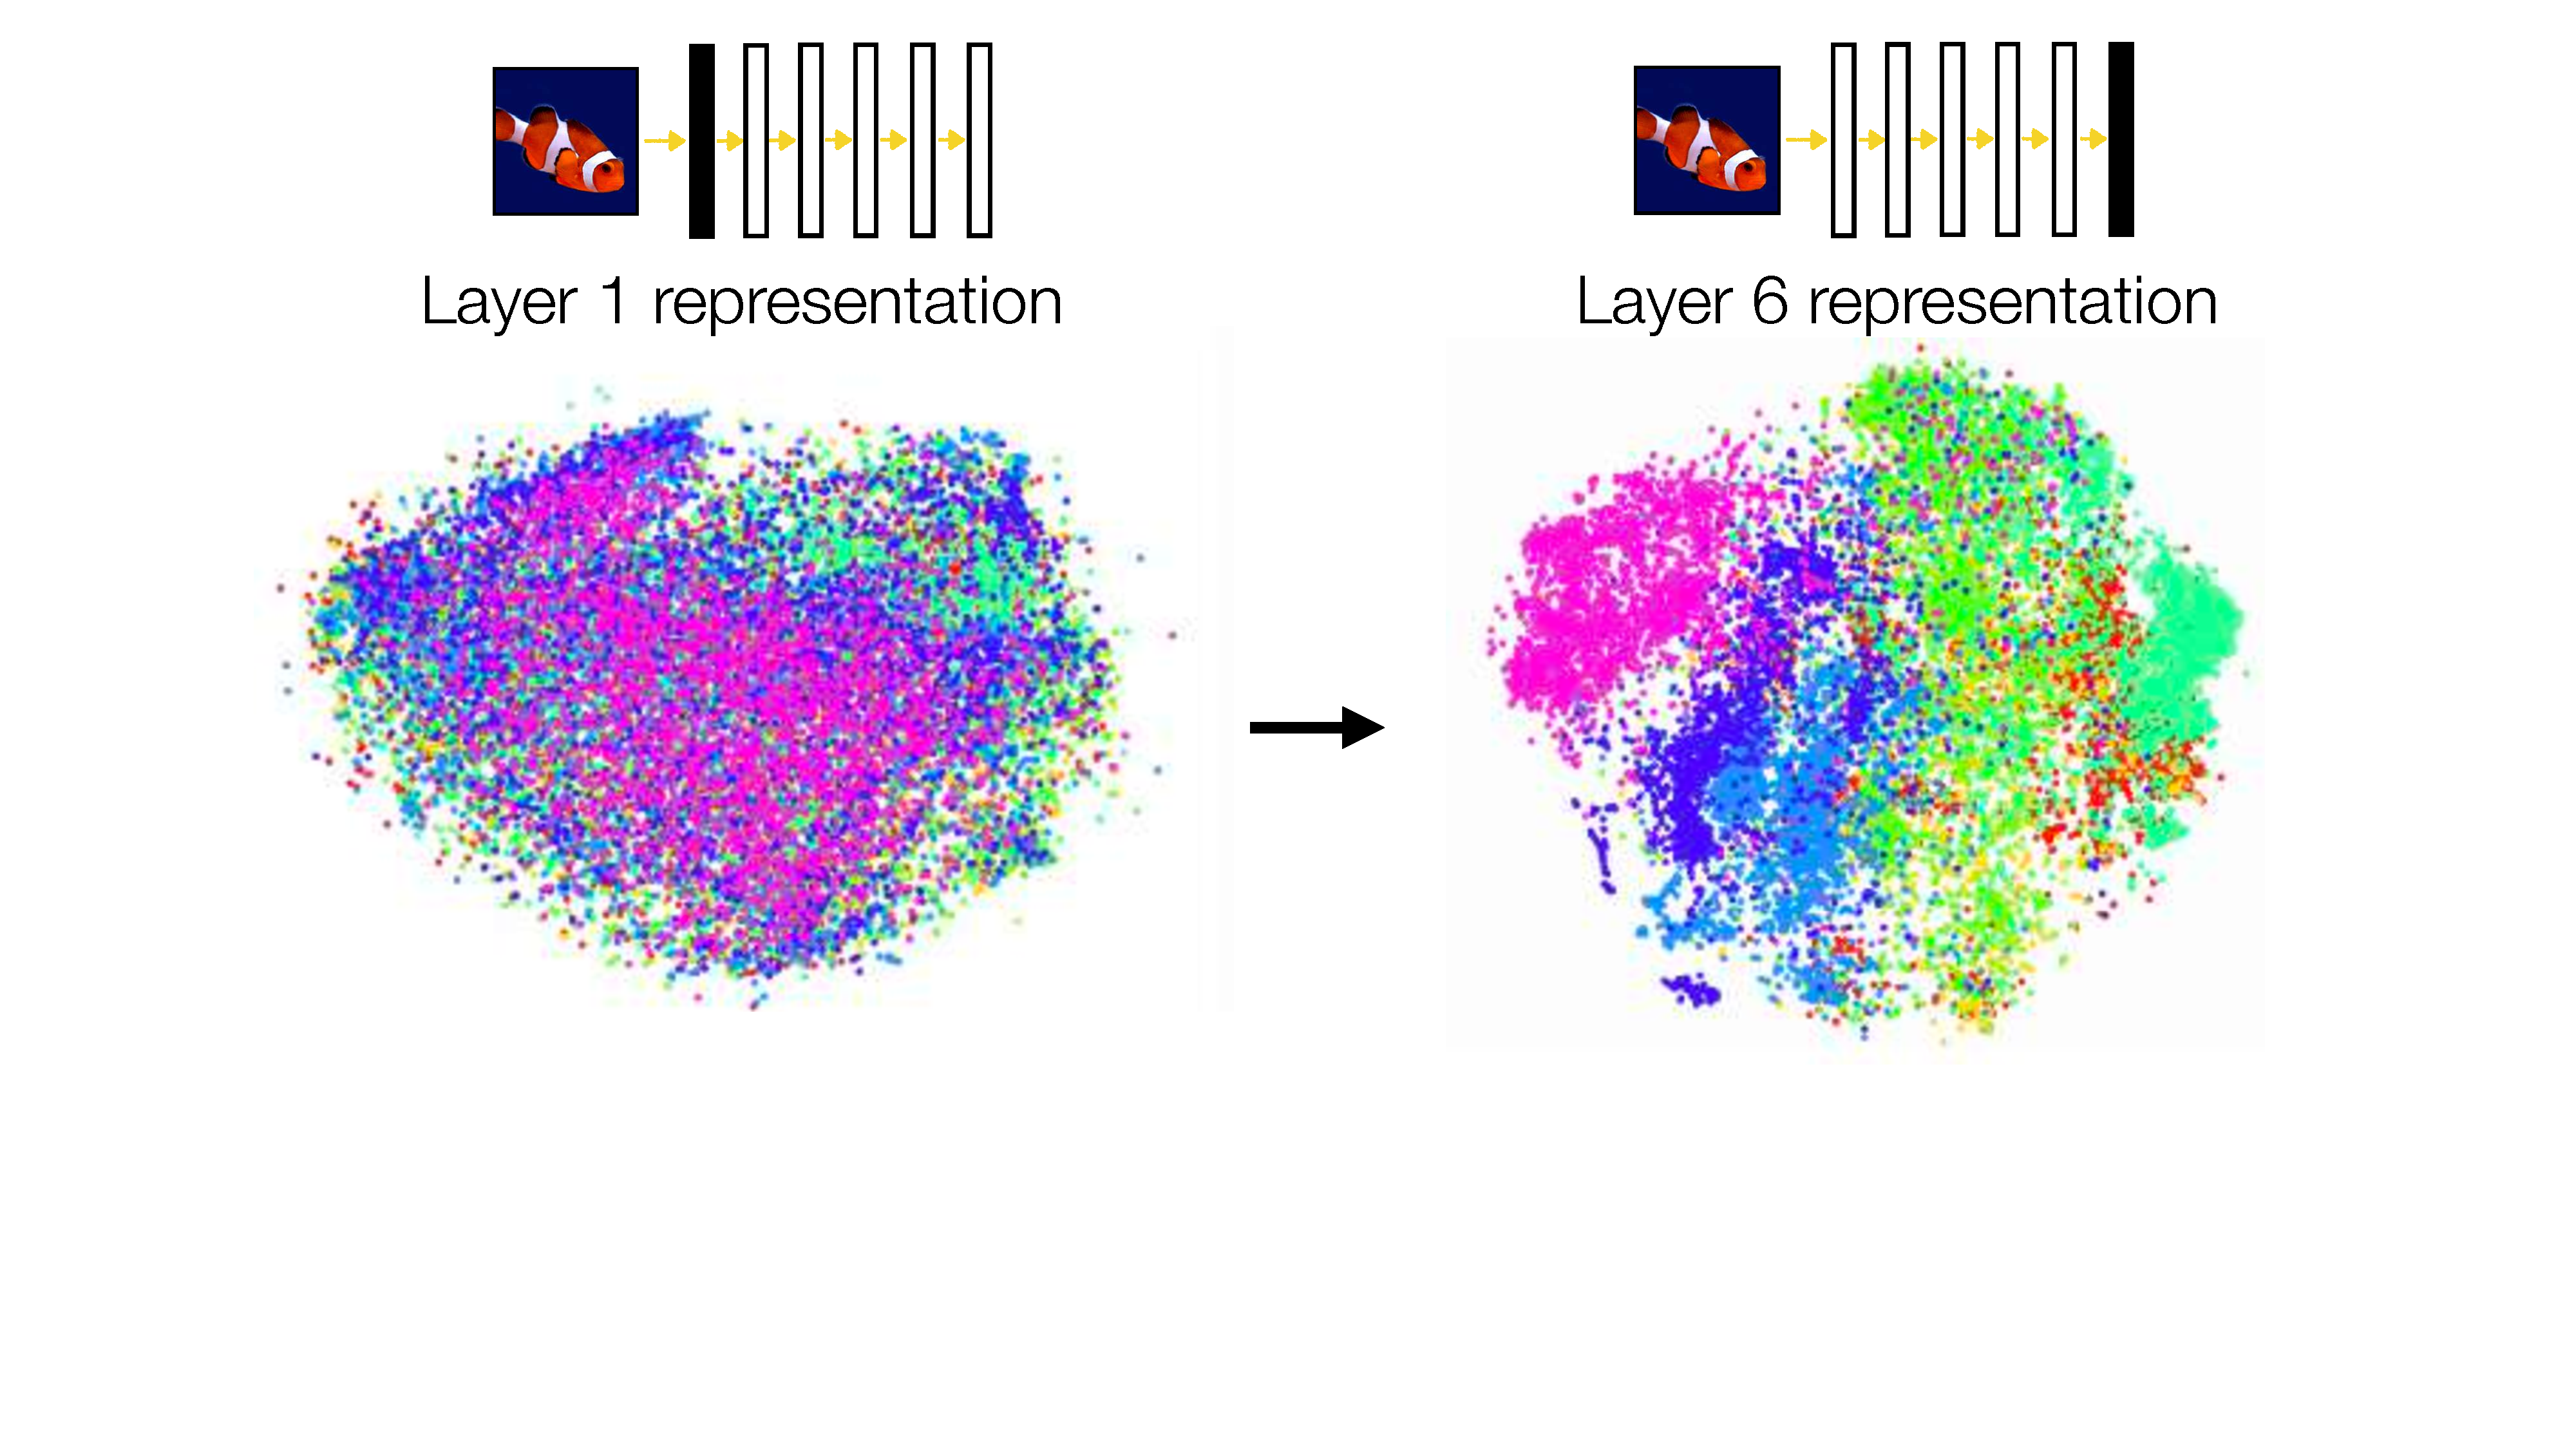
\includegraphics[width=0.6\linewidth]{./figures/neural_nets/decaf_tsne.pdf}
%     }
%     \caption{How a deep image classifier remaps input pixels into a disentangled representation where semantic classes are separated. The t-SNE visualization is taken from \cite{decaf}. \reviewcomment{Replace fish photo, get permission to use tsne image.}}
%     \label{fig:neural_nets:decaf_tsne}
% \end{figure}
\begin{figure}[t]
    \centerline{
    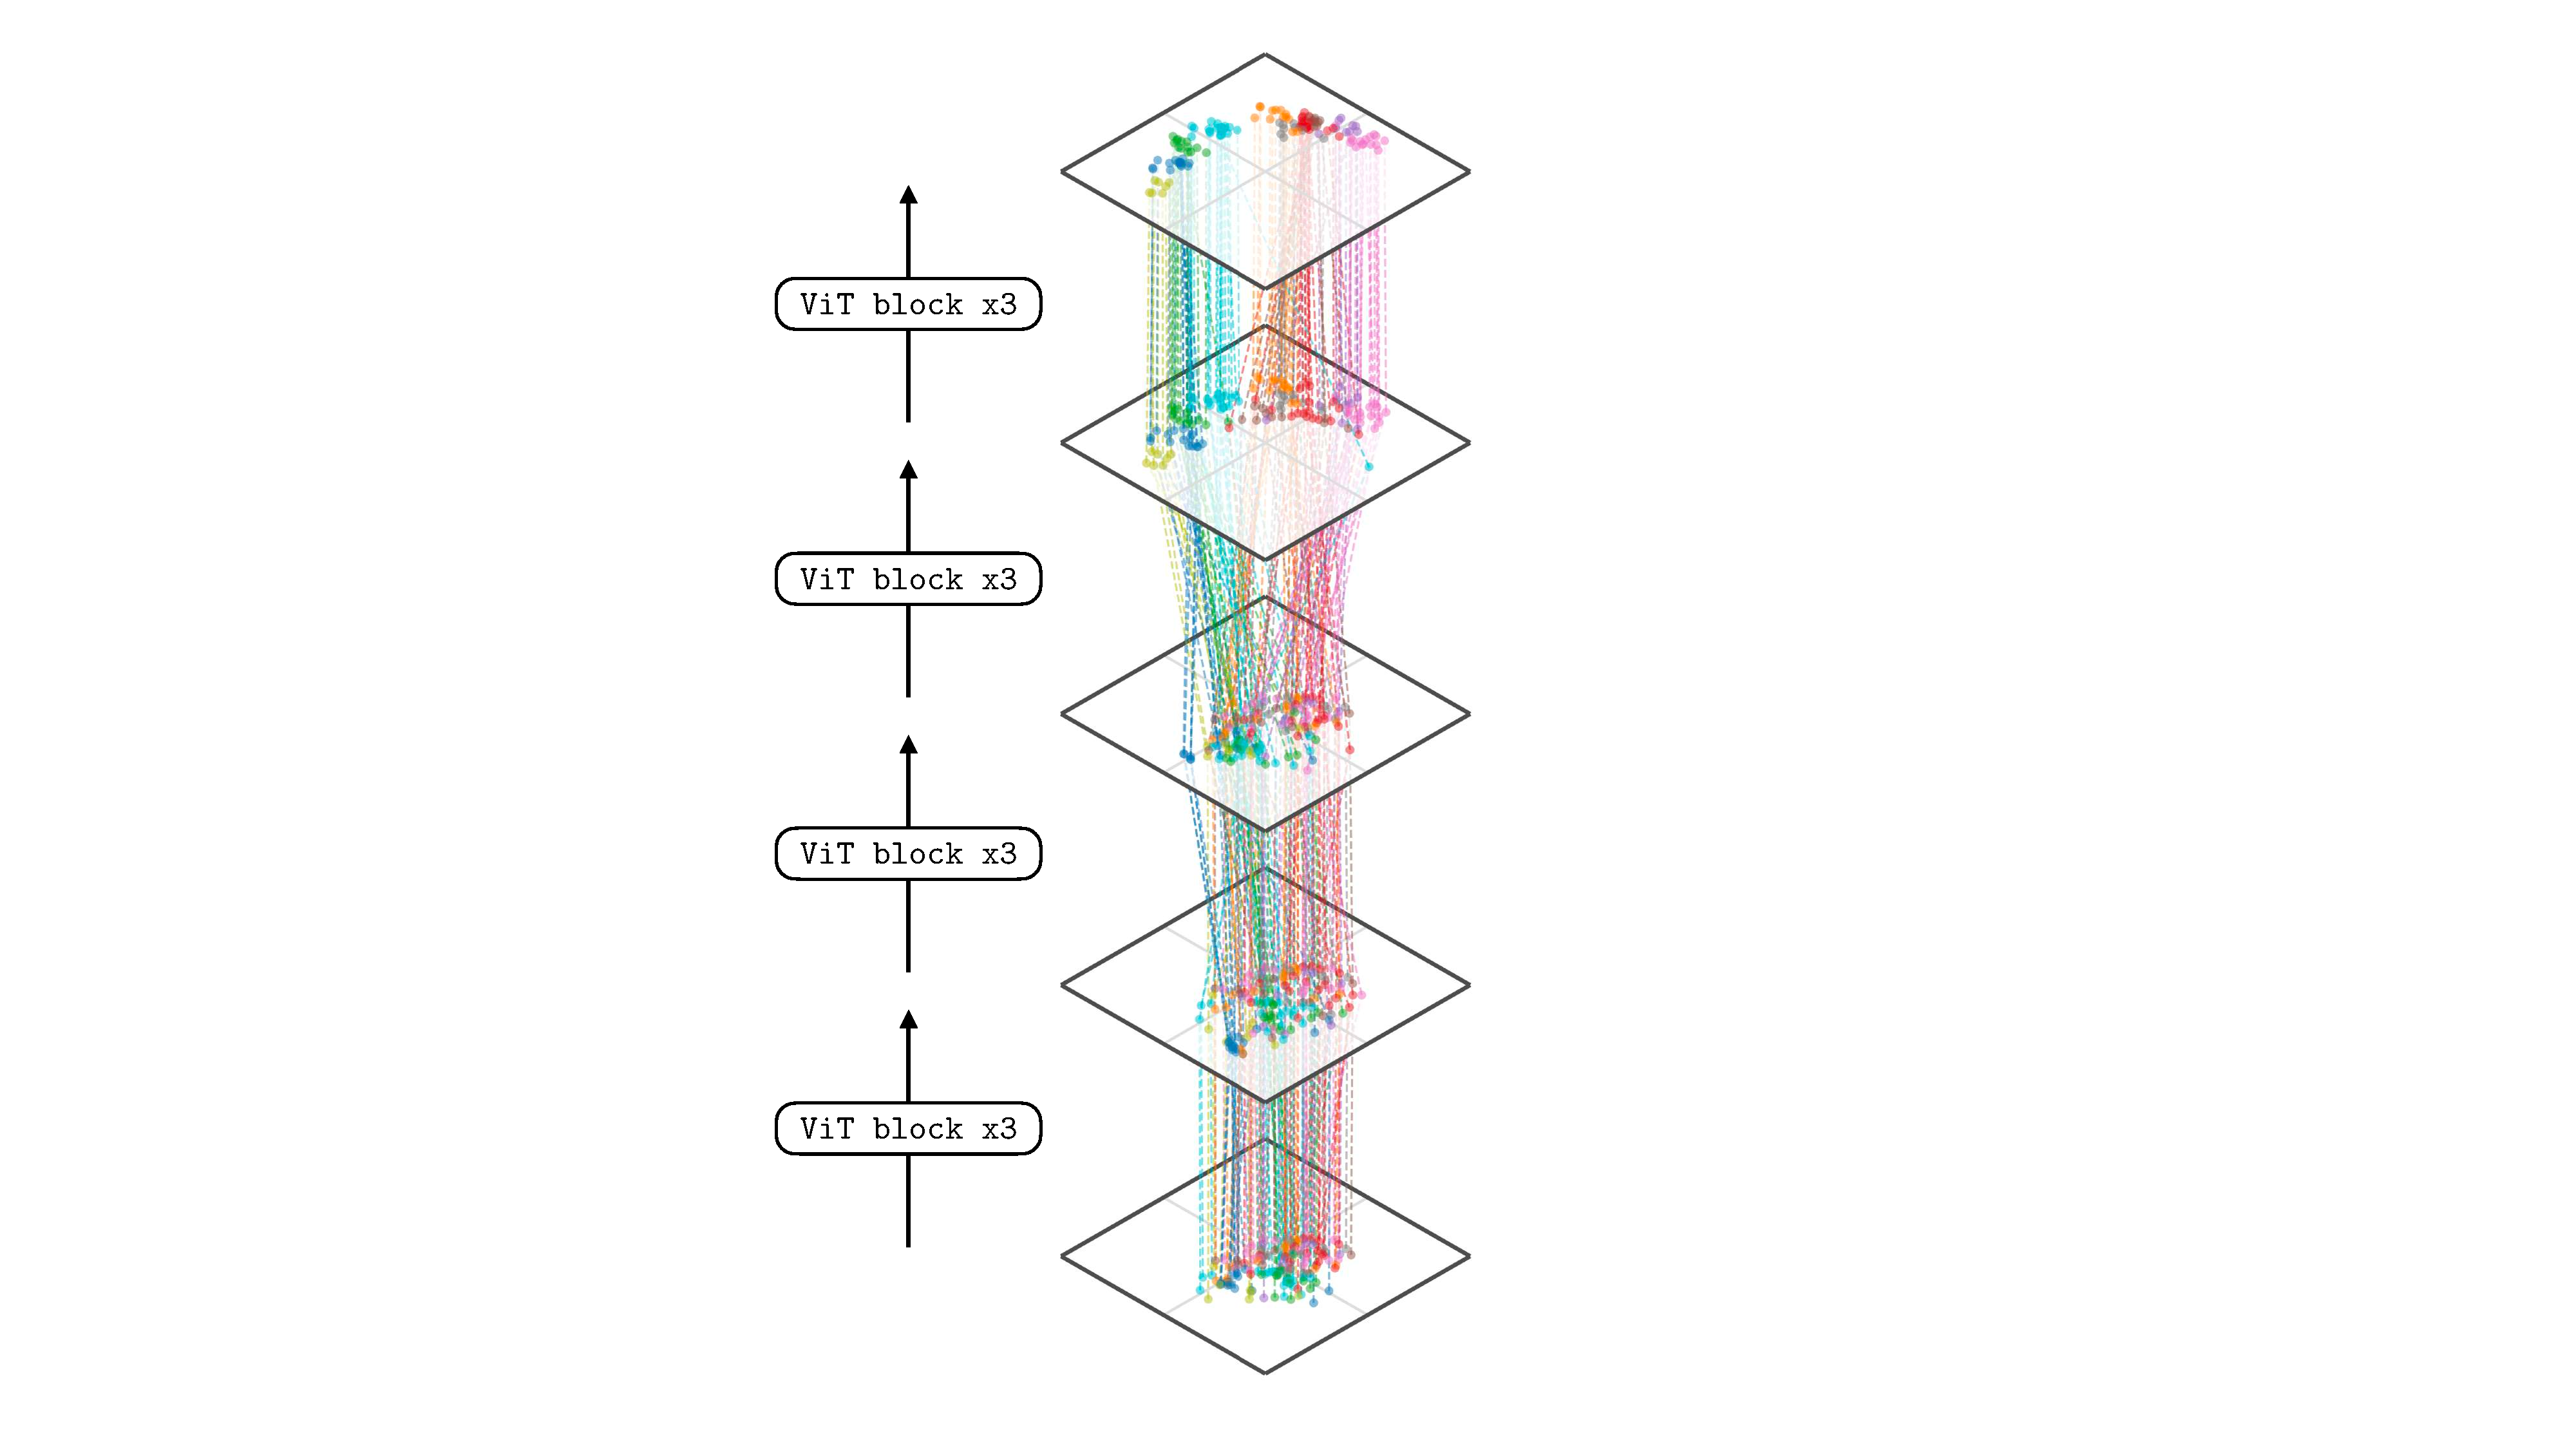
\includegraphics[width=0.375\linewidth]{./figures/neural_nets/vit_mapping_plot.pdf}
    }
    \caption{How a powerful deep net remaps input images into a disentangled representation where semantic classes (shown in different colors) are separated. This deep net is a vision transformer (ViT~\cite{dosovitskiy2020vit}), which we will learn about in \sect{\ref{sec:transformers:ViT_arch}}. It was trained using contrastive language-image pre-training (CLIP~\cite{radford2021learning}, see \sect{\ref{sec:VLMs:CLIP}}). Each \texttt{ViT block} contains multiple layers of neural processing (see \fig{\ref{fig:transformers:ViT_arch}}; we visualize the embeddings right after the first \texttt{token norm} in a block). We apply t-SNE jointly across all shown layers.} %which is size $(NL) \times d$, where $N$ is the number of images, $L$ is the number of layers that are plotted, and $d$ is the dimensionality of each layer (how many neurons it has).}
    \label{fig:neural_nets:vit_mapping_plot}
\end{figure}

Notice that on the first layer, semantic classes are not well separated but by the last layer the representation has {\bf disentangled} the semantic classes so that each class occupies a different part of representational space. This is expected because the final layer in this visualization is near the output of the network, and this network has been trained to output a direct representation of semantics (in particular, this net was trained with contrastive language-image pre-training [CLIP~\cite{radford2021learning}], which is a method for learning semantic representations that we will learn about in \sect{\ref{sec:VLMs:CLIP}}).%, that is, a completely disentangled representation.

\section{Concluding Remarks}
Layer by layer, deep nets transform data from its raw format to ever more abstracted and useful representations. It can be helpful to think about this process as a set of geometric transformations of a data distribution, or as a kind of disentangling where initially messy data gets reorganized so that different data classes become cleanly separated.